\chapter{Enabling Next Generation Small-Scale Dynamo Simulations}
\label{chapter:quokka}

\noindent\hfill\parbox{0.75\textwidth}{\raggedleft
This chapter is adapted from a manuscript in preparation:
\textit{Kriel, N., Cole-Kodikara, E., Wibking, B., Krumholz, M. R., He, C.-C., Sarkar, A., \& Li, P. S. Magnetising the \textsc{Quokka} code with fast, second-order accurate, error-correcting schemes for ideal magnetohydrodynamics on GPUs.}
}\par

\section{Chapter Abstract}

We implement a second-order accurate constrained transport (CT) ideal magnetohydrodynamics (MHD) module in the open-source, adaptive mesh refinement code \textsc{Quokka}. As part of this implementation we introduce and test two significant methodological innovations. The first is a flux correction strategy that improves stability by locally and self-consistently falling back to a more dissipative, first-order in space and time scheme in regions where the higher-order update would produce an unphysical state; the second is a new method for reconstructing electromotive forces (EMFs) at cell edges -- a necessary part of any CT-MHD scheme. We carry out a systematic comparison between our new scheme and two existing state-of-the-art methods for EMF reconstruction from \citet{Felker18a} and \citet{Balsara25b}. We find that all schemes recover solutions of comparable accuracy, but that our new scheme is $1.6\times$ and $1.3\times$ faster on GPU architectures, respectively, albeit with somewhat reduced stability in the most challenging non-linear problems. We show that our new scheme provides excellent results for a wide range of standard MHD tests, and that with it, \textsc{Quokka} achieves $>50$ million cell updates per GPU per second.

\section{Chapter Introduction}

\textsc{Quokka} is a new, open-source, GPU-accelerated radiation-hydrodynamics code aimed at modelling radiating, highly compressible flows across a wide range of scales \citep[hereafter \citetalias{Wibking22a}]{Wibking22a}. In this paper we extend \textsc{Quokka} to include an ideal magnetohydrodynamics (MHD) module, and in the process test a broad combination of Riemann solvers, constrained-transport (CT) schemes, and error-correction strategies -- some previously-published and some new to this work -- in order to identify ones that offer a good combination of accuracy and performance in these complex flow regimes. This comparison of available approaches in the literature will not only inform our design choices for implementing MHD into \textsc{Quokka}, but we anticipate that it will also be directly useful to others implementing MHD in similar GPU-oriented codes. To this end, the remainder of this Introduction will be dedicated to first situating \textsc{Quokka} within the broader landscape of astrophysical simulation codes, before we turn to the numerical challenges posed by highly compressible MHD flows, which \textsc{Quokka} aims to simulate.

\subsection{Why \textsc{Quokka}?}

While a number of mature grid-based codes already provide rich multiphysics capabilities for galaxy formation and the interstellar medium (ISM), including \textsc{Athena++} \citep{Stone20a}, \textsc{Enzo} \citep{Bryan14a}, \textsc{Flash} \citep{Fryxell00a}, \textsc{Orion} \citep{Li21b}, \textsc{Pencil} \citep{Brandenburg02a}, and \textsc{Ramses} \citep{Teyssier02a}, these codebases are primarily CPU-based, with GPU support still an active area of development. There are also newer codes like \textsc{Cholla} \citep{Schneider15a} and \textsc{AthenaK} \citep{Stone24a} that were developed from the outset for GPU architectures, and already include MHD solvers. However, they lack many of the multiphysics features required for simulations of galaxies, star formation, and ISM physics more broadly. For example, \textsc{AthenaK} focuses on applications in high-energy astrophysics, and therefore does not provide modules for ISM cooling, star formation, or stellar feedback, and only includes radiative transfer for relativistic flows. Similarly,  while \textsc{Cholla} does include ISM-relevant cooling, it does not include either radiative transfer or self-consistent star formation and feedback, and also does not provide adaptive mesh refinement (AMR), a crucial capability for simulations of collapse in self-gravitating flows. Taken together, this highlights a gap in the current code landscape: there is a lack of GPU-native, AMR-enabled codes that combine non-relativistic radiation-hydrodynamics with the broader multiphysics required for ISM and star-formation applications.
    
\textsc{Quokka} attempts to bridge this gap. It is a GPU-native\footnote{
    \textsc{Quokka} can also be built and run on CPU-only systems.
} radiation-hydrodynamics code built on \textsc{AMReX} \citep{Zhang19b}, designed for high-resolution AMR studies of non-relativistic, radiating, compressible flows. Recently, the codebase has grown to include a broader set of physics modules, including multi-group, non-relativistic radiation transport \citep{He24a, He24b}, complex gas-particle interactions \citep{He25a}, and subgrid models aimed at ISM, circumgalactic, and star-formation applications, which has been successfully deployed in simulations of galactic winds launched by supernovae \citep{Vijayan24a, Vijayan25a}. However, what \textsc{Quokka} has lacked so far is the ability to simulate magnetised flows, so one goal of this paper is to add and test this capability.

\subsection{Design considerations for highly compressible MHD}
\label{sec:intro:goals}

The systems that \textsc{Quokka} was designed to model -- from flows during cosmological structure formation and galaxy assembly, to star-forming interstellar gas, protostellar and protoplanetary discs, and planetary flows -- are highly compressible, with dynamics that evolve over a wide range of spatial and temporal scales. In these environments the sonic Mach number $\mathcal{M}$ (flow speed relative to the sound speed), Alfv\'en Mach number (relative to the Alfv\'en speed), and plasma-$\beta$ (gas-to-magnetic pressure ratio) can each vary by many orders of magnitude. The gas in these systems is also often at least partially ionised, leading to dynamically important magnetic fields threading these flows. A code that aims to explore these regimes must therefore satisfy several competing requirements: it must be (i) robust in the presence of high-$\mathcal{M}$ flows and strong shocks, (ii) accurate enough to capture low-$\mathcal{M}$, instability-driven dynamics, and (iii) scalable to very high resolutions on modern hardware, particularly on GPUs, and often in combination with AMR.

A common strategy for satisfying these challenges is to use a Godunov finite-volume scheme \citep{Toro97a}. This is the approach adopted by \textsc{Quokka}, where conserved quantities are stored as cell averages and updated through fluxes across cell interfaces. In such a scheme one collects the evolved fields into a conservative state vector $\mVector{S}_\mathrm{c}$ obeying
\begin{align}
    \mppFrac{\mVector{S}_\mathrm{c}}{t}
        + \nabla\cdot\mVector{F}\sbrac{\mVector{S}_\mathrm{c}}
        &= \mVector{G}\sbrac{\mVector{S}_\mathrm{c}}
    , \label{eqn:conservative_form}
\end{align}
where $\mVector{F}[\mVector{S}_\mathrm{c}]$ provides the fluxes of conserved quantities, and $\mVector{G}[\mVector{S}_\mathrm{c}]$ collects explicit sources and sinks (\eg gravity and radiation couplings). Integrating over cell volumes $\mathcal{V}$, one obtains the semi-discrete evolution equation
\begin{align}
    \mppFrac{}{t} \langle \mVector{S}_\mathrm{c}\rangle_\mathcal{V}
        + \frac{1}{|\mathcal{V}|} \int_{\partial\mathcal{V}}
            \mVector{F} \cdot \mVectorUnit{n}
       \, \mathrm{d} A
        &= \langle \mVector{G} \rangle_\mathcal{V}
    , \label{eqn:godunov:integral}
\end{align}
where
\begin{align}
    \langle \mVector{S}_\mathrm{c}\rangle_\mathcal{V}
        \equiv \frac{1}{|\mathcal{V}|} \int_\mathcal{V}
            \mVector{S}_\mathrm{c}
       \, \mathrm{d} V
\end{align}
is the average value of $\mVector{S}_\mathrm{c}$ over a cell volume (and a similar definition follows for $\langle\mVector{G}\rangle_\mathcal{V}$) and $\partial\mathcal{V}$ is the surface of the cell face, with area $A$. The second term on the left-hand side of \autoref{eqn:godunov:integral} follows from the divergence theorem, and for cuboid cells (as used in \textsc{Quokka}) this integral can be expressed as a sum over the area-averaged fluxes across the six faces adjoining each cell and its neighbours. It then follows that, because these interfaces in turn each carry a single flux that leaves one cell and enters its neighbour, conservation is enforced by construction.

Schemes in this family have proven very robust for handling strong shocks, with higher-order accuracy still attainable in smooth flows \citep{kritsuk2011comparing}. Moreover, because Godunov schemes operate directly on the conserved variables, it is straightforward to extend to AMR. The main numerical choices then lie with how one approximates the face-averaged fluxes, which typically involves (i) reconstructing interface states from the cell averages and (ii) solving a local Riemann problem to obtain an upwinded flux. Different choices represent different trade-offs between stability, accuracy, and computational cost.

In ideal MHD the conservative system can be written compactly\footnote{
    Here, and throughout this paper, we adopt the usual rationalised-Gaussian unit system whereby all non-magnetic quantities are in CGS units and the magnetic field $\mVector{b}$ is expressed in units of Gauss divided by $\sqrt{4\pi}$.
} as
\begin{align}
    \mppFrac{}{t}\begin{Bmatrix}
            \rho \\
            \rho\mVector{u} \\
            e_\mathrm{tot} \\
            \mVector{b}
        \end{Bmatrix}
            = -\nabla\cdot\begin{Bmatrix}
                \rho\mVector{u} \\
                \rho(\mVector{u}\otimes\mVector{u})
                    + \rbrac{p + b^2/2} \mTensor{I}
                    - \mVector{b}\otimes\mVector{b} \\
                \rbrac{e_\mathrm{int} + p + b^2/2}\mVector{u}
                    - (\mVector{u}\cdot\mVector{b})\, \mVector{b} \\
                \mVector{u}\otimes\mVector{b}
                    - \mVector{b}\otimes\mVector{u}
            \end{Bmatrix}
    , \label{eqn:mhd_system}
\end{align}
since there are no explicit source or sink terms in ideal MHD. Here $\rho$, $\mVector{u}$, and $\mVector{b}$ are the fluid density, fluid velocity, and magnetic field, respectively, with total energy density $e_\mathrm{tot} = e_\mathrm{int} + (1/2)\rbrac{\rho u^2 + b^2}$, and internal energy $e_\mathrm{int}$; here, also, $b^2 \equiv \mVector{b}\cdot\mVector{b}$ and $\otimes$ is the tensor (or outer) product such that, for example, $\mVector{b}\otimes\mVector{u} \equiv b_i u_j$ in index notation.

On the surface, this system of equations might look like a straightforward extension of the Euler system (\ie inviscid hydrodynamics), which may lead one to naively assume that evolving \autoref{eqn:mhd_system} in a Godunov framework simply requires the hydro-Riemann solver be replaced with an MHD-aware Riemann solver. However, magnetised flows face a unique constraint that is not automatically satisfied by a standard Godunov scheme: the numerical method must respect $\nabla\cdot\mVector{b} = 0$. This is not guaranteed for a purely cell-centred flux update of $\mVector{b}$, which is a well known numerical problem to which many approaches have been attempted \citep{kritsuk2011comparing}, including the development of CT methods \citep{Evans88a}.

In many ways CT can be viewed as a natural extension of the Godunov approach to magnetic fields on Cartesian meshes, where, rather than evolving cell-averaged components of $\mVector{b}$ from face fluxes, one instead evolves face-averaged normal-components of $\mVector{b}$ from edge-centred electromotive forces (EMFs) in a way that preserves the discrete divergence by construction. This follows from the central fact that, for ideal MHD, the magnetic field evolves according to the induction equation
\begin{align}
    \mppFrac{\mVector{b}}{t}
        &= -\nabla\times\mVector{\varepsilon}
    , \label{eqn:induction_intro}
\end{align}
where $\mVector{\varepsilon} = -\mVector{u}\times\mVector{b}$ is the ideal EMF. Integrating the normal component of \autoref{eqn:induction_intro} over a cell face $\partial\mathcal{V}$ with unit normal direction $\mVectorUnit{n}$, gives
\begin{align}
    \int_{\partial\mathcal{V}} \mppFrac{\mVector{b}}{t}\cdot\mVectorUnit{n}\, \mathrm{d} A
        &= -\int_{\partial\mathcal{V}}
            \rbrac{\nabla\times\mVector{\varepsilon}}
            \cdot\mVectorUnit{n}\, \mathrm{d} A
    . \label{eqn:step:integrate-dbdt}
\end{align}
Commuting the time derivative on the left-hand side motivates the definition of the face-averaged normal field,
\begin{align}
    \langle{b_n}\rangle_{\partial\mathcal{V}}
        &\equiv \frac{1}{|\partial\mathcal{V}|}
            \int_{\partial\mathcal{V}}
            \mVector{b}\cdot\mVectorUnit{n}\, \mathrm{d} A
    ,
\end{align}
while Stokes' theorem converts the surface integral of the curl, on the right-hand side of \autoref{eqn:step:integrate-dbdt}, into a circulation (\ie closed line integral) of the EMF around the face boundary $\partial\mathcal{A}$, giving the semi-discrete evolution equation
\begin{align}
    \mppFrac{}{t}\langle{b_n}\rangle_{\partial\mathcal{V}}
        &= -\frac{1}{|\partial\mathcal{V}|}
            \oint_{\partial\mathcal{A}}
            \mVector{\varepsilon}\cdot\mathrm{d}\mVector{\ell}
    . \label{eqn:ct_stokes_intro}
\end{align}
CT is then a discrete realisation of \autoref{eqn:ct_stokes_intro}, in which $\mVector{b}$ is stored directly as face-averaged normal components, and EMFs as edge-averaged tangential components. From this, the magnetic update is obtained by approximating the line integral (in \autoref{eqn:ct_stokes_intro}) as a sum of tangential EMF components over the four face edges. With this staggering, each edge EMF contributes to exactly two neighbouring face updates with opposite sign, so the discrete divergence (defined by the oriented sum of face-averaged fluxes over the cell boundary) is preserved by construction; $\nabla\cdot\mVector{b}$ is conserved over the discrete stencil (to numerical precision), and so, if it is initially zero, then it remains zero up.

With this context, it then follows that enabling ideal MHD in \textsc{Quokka}  amounts to extending its finite-volume flux update in two coupled ways. First, we replace the purely hydrodynamic flux function with an MHD-aware Riemann solver. From the cell-averaged conserved variables we reconstruct left and right states at cell faces and solve the corresponding MHD Riemann problem to obtain upwinded, face-centered fluxes for the conservative update of cell-centred quantities. Second, we compute the magnetic update using CT. In the sections that follow we will describe our choice of MHD-aware Riemann solver and suite of CT schemes.

\subsection{Outline of this paper}

The remainder of this paper is organised as follows. In \autoref{sec:method} we present the new ideal MHD module, describing the set of (Riemann and CT) solvers, interpolation schemes, and flux correction schemes that we implement. In \autoref{sec:performance} we compare the accuracy and performance of these different schemes, before recommending our preferred scheme combination for \textsc{Quokka}. In \autoref{sec:tests} we then compare our recommended scheme against a more comprehensive set of MHD tests, and then finally summarise our findings and discuss future extensions of MHD for \textsc{Quokka} in \autoref{sec:conclusions}. Because in what follows we will need to track quantities with many different types of indices -- indicating grid position, time, direction, etc., we will use notation as described in \autoref{sec:notation}.

\section{Numerical implementation}
\label{sec:method}

Here we introduce the different parts of our MHD scheme (summarised in \autoref{fig:schematic:flowchart}). We first describe the mesh\footnote{
    In addition to the ideal MHD variables described below, \textsc{Quokka} also supports a dual-energy formalism, in which the internal energy is evolved alongside the total energy, and (optionally) passive scalars. These quantities trivially augment the conservative state vector, $\mVector{S}_\mathrm{c}$, with extra cell-centred quantities. For clarity, however, we restrict the discussion in this paper to the minimal set of conserved variables relevant for ideal MHD.
    \label{fnote:dual-energy}
} we use to discretise the equations in \autoref{sec:methods:mesh}. We then describe the method we use to compute the fluxes of cell-centred variables in \autoref{sec:methods:flux}, and to compute EMFs for the face-centred magnetic fields in \autoref{sec:methods:emf}. We explain how we chain these calculations together within our overall time-stepping scheme, including our implementation of flux correction, in \autoref{sec:methods:time-stepping}, and in \autoref{sec:methods:amr} we conclude with a discussion of how the scheme was extended to AMR.

\subsection{Mesh}
\label{sec:methods:mesh}

\begin{figure}
    \centering
    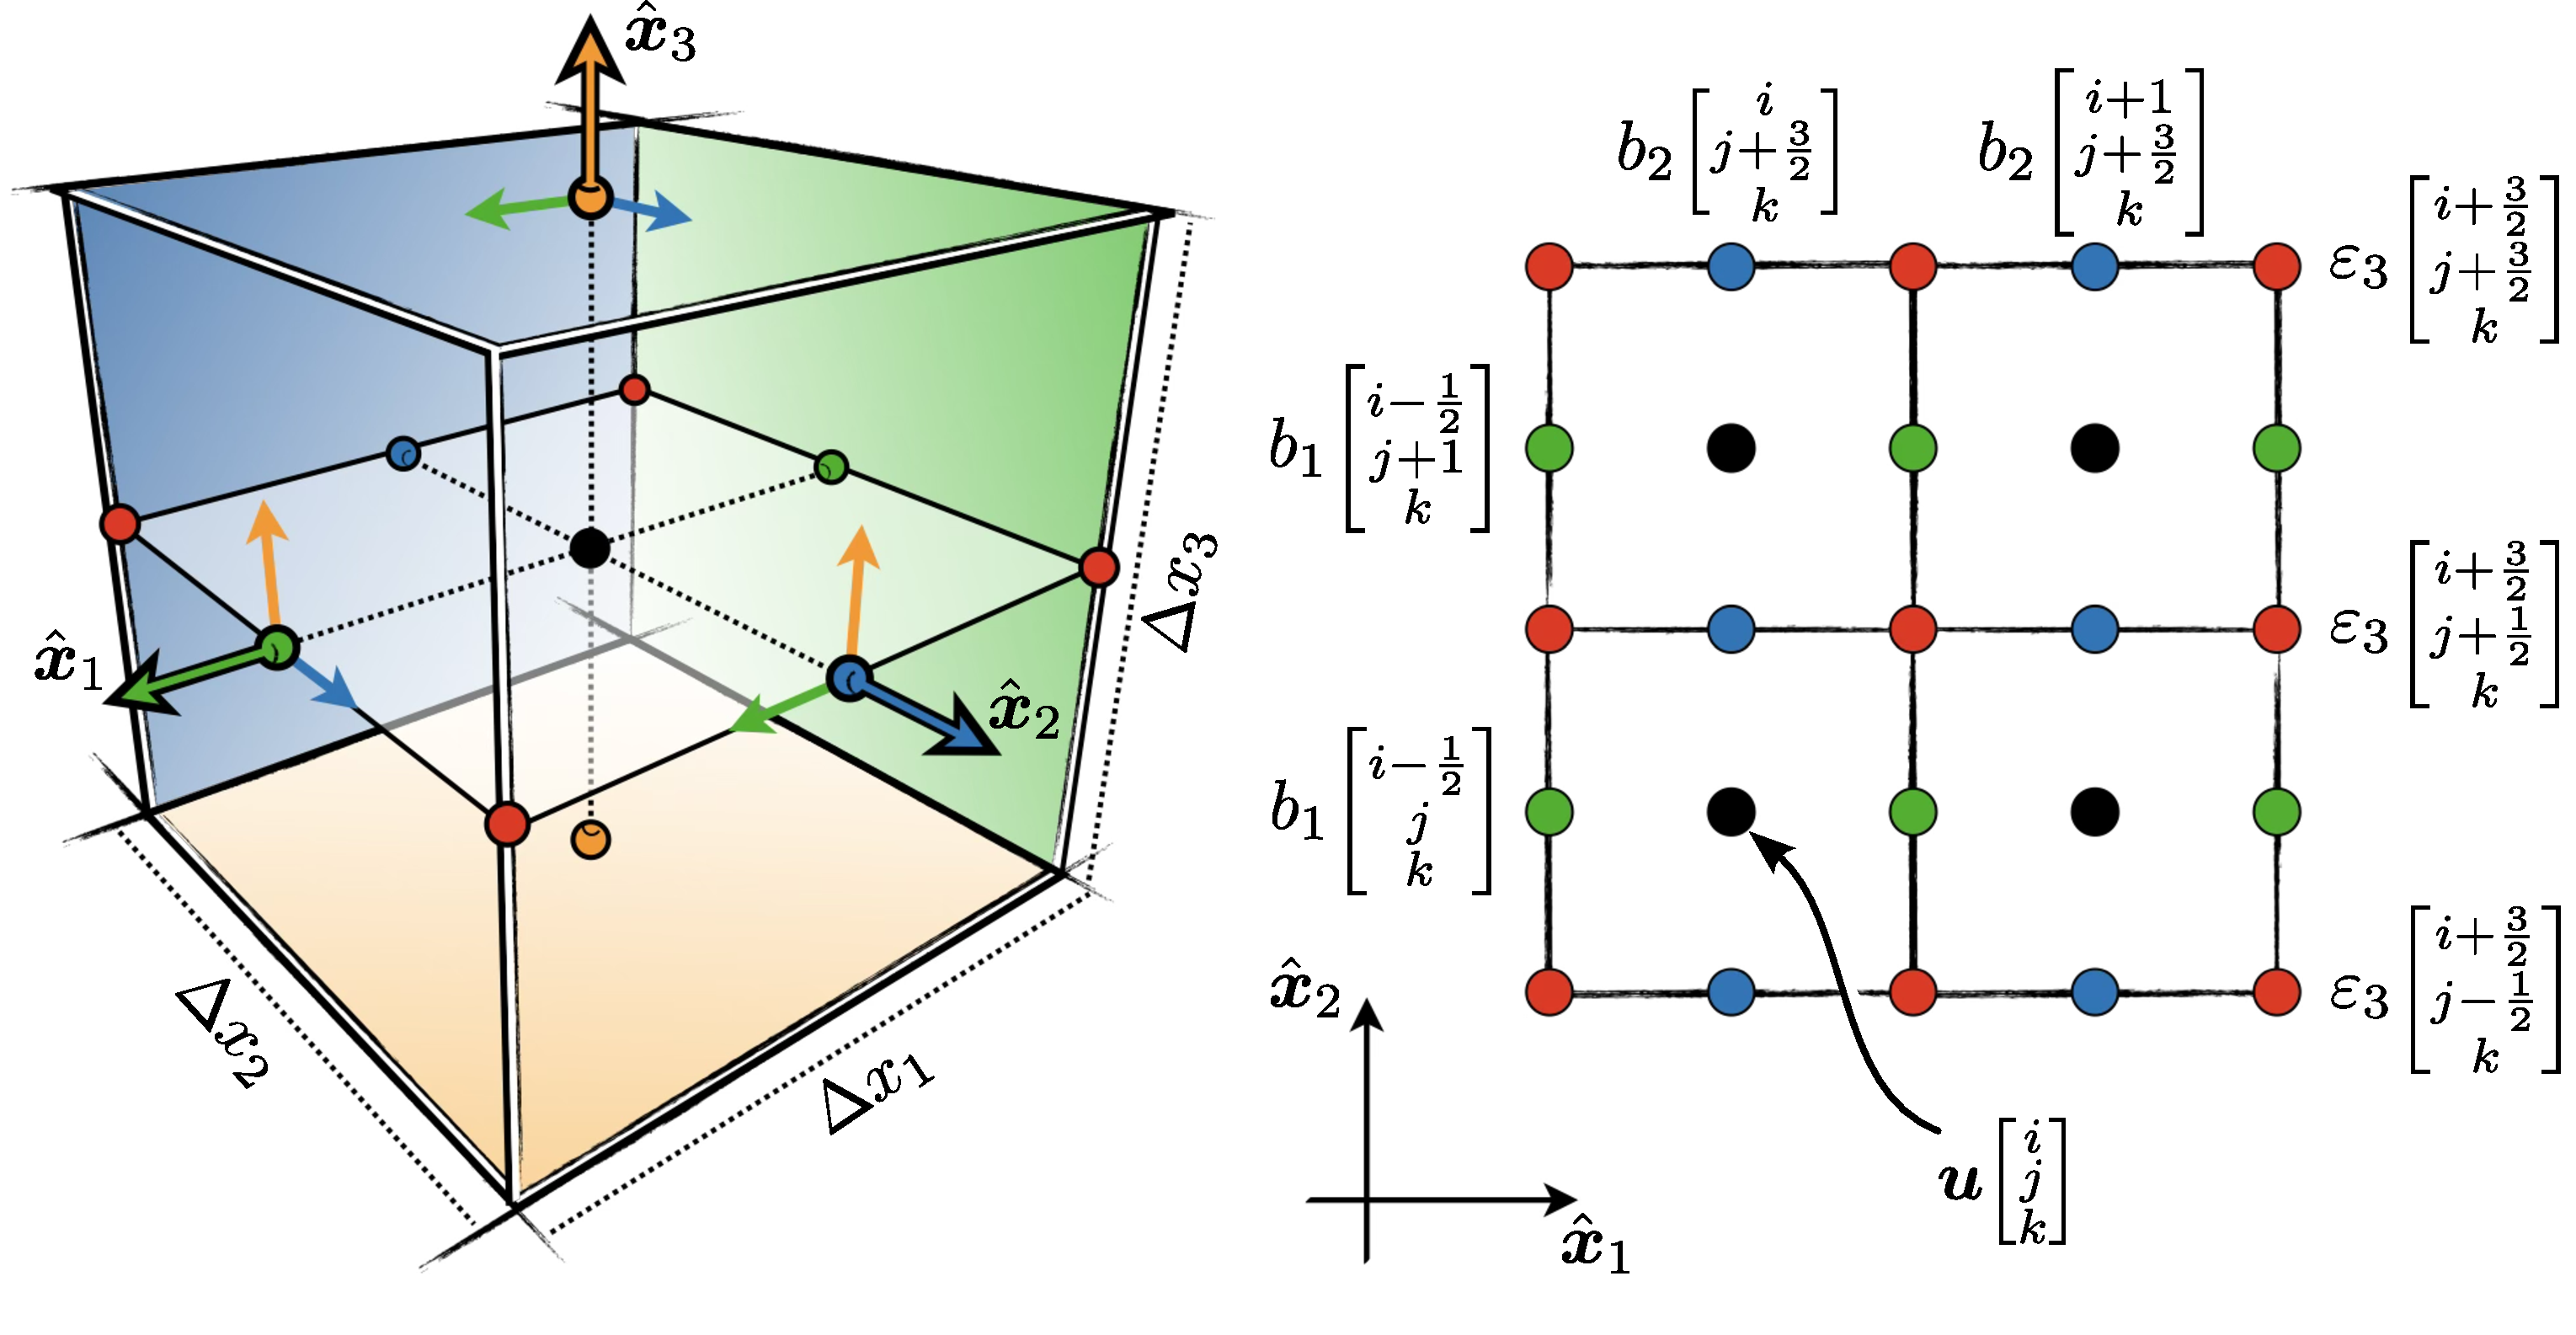
\includegraphics[width=\linewidth]{figures/quokka-mhd/schematics/grid.pdf}
    \caption{The \textsc{Quokka} mesh shown in perspective view (left) and a slice in the $(x_1,x_2)$-plane (right). All non-magnetic conserved and primitive variables, for example the fluid velocity $\mVector{u}$, are stored at cell centres (black points), denoted by integer indices $ijk$. The three components of the magnetic field are stored at faces corresponding to their direction (blue, green, and orange points for the faces in the $x_1$, $x_2$, and $x_3$ directions) with one half-integer index and two integer indices; thus for example $b_1$ is stored at $(i - 1/2,j,k)$ and $b_2$ at $(i,j - 1/2,k)$. Finally, the three components of the EMF $\mVector{\varepsilon}$ are stored at cell edges (red points) with two half-integer indices and one integer index, with the direction of the EMF component parallel to the direction of the cell edge; thus for example $\varepsilon_3$ is stored at $(i - 1/2,j - 1/2,k)$.}
    \label{fig:schematic:grid}
\end{figure}

Our implementation uses the staggered mesh scheme first introduced for astrophysical MHD by \citet{Evans88a}, which had precursors in other MHD fields \citep[\eg][]{Yee66a, Brecht81a}; today, this approach is standard in essentially all three-dimensional CT schemes \citep[\eg][]{Fromang06a, Gardiner08a, Li12a}. As illustrate in \autoref{fig:schematic:grid}, we store all the conserved quantities except for magnetic fields at cell centres, and thus our vector of conserved cell-centred quantities is
\begin{align}
    \mVector{S}_\mathrm{c}\EvalAtH{i}{j}{k}
        = \begin{Bmatrix}
            \rho\EvalAtH{i}{j}{k} \\
            \rho\EvalAtH{i}{j}{k} \mVector{u}\EvalAtH{i}{j}{k} \\
            e_\mathrm{tot}\EvalAtH{i}{j}{k}
        \end{Bmatrix}
    , \label{defn:state-vector}
\end{align}
where we use integer indices $i$, $j$, and $k$ to denote cell-centred quantities. Each of these quantities should be understood as an average over cell $(i, j, k)$, but for compactness we will omit the angle bracket notation used in \autoref{eqn:godunov:integral} from this point forward. Moreover, for clarity, we define $\mVector{S}_\mathrm{c}$ here for the minimal ideal-MHD system, and note that our dual-energy and passive-scalar extensions correspond with extra cell-centred components (see footnote \ref{fnote:dual-energy}).
 
We store the magnetic field on cell faces, with the component normal to a face stored at the face centre (see \autoref{fig:schematic:grid}). Thus $b_1$ is indexed as $\,\EvalAtH{i + 1/2}{j}{k}$, $b_2$ as $\,\EvalAtH{i}{j + 1/2}{k}$, and $b_3$ as $\,\EvalAtH{i}{j}{k + 1/2}$. In general, a half-integer index together with two integer indices corresponds with a face-centred quantity that has been face-averaged. We also use edge-centred quantities which is associated with two half-integer indices, for example $\EvalAtH{i + 1/2}{j + 1/2}{k}$, which indicates an edge-averaged values.

% Our implementation also supports the use of a dual energy formalism, in which we treat the internal energy as a quantity distinct from the total energy, and the use of passive scalars to represent mass fractions of different species. Either of these options adds additional conserved quantities to the state vector $\mVector{S}_\mathrm{c}$. For simplicity, however, we will limit our discussion here to the case where the only conserved quantities are the five listed in \autoref{defn:state-vector}. Extension to additional conserved quantities is no different for MHD than it is for hydrodynamics.

\subsection{Flux calculation}
\label{sec:methods:flux}

As discussed in \autoref{sec:intro:goals}, the first required step for a Godunov scheme for ideal MHD is a recipe to compute the fluxes of the cell-averaged quantities across cell faces. This step in turn has two parts: an interpolation scheme used to compute interface states on either side of the face, and a Riemann solver to compute fluxes from those interface states.

For the interpolation part of the scheme, our approach closely follows the one \textsc{Quokka} uses for pure hydrodynamics, as described in \citetalias{Wibking22a}. Thus here we only summarise and identify points of difference necessitated by the inclusion of magnetic fields. We first convert our vector of conserved variables to a vector of cell-centred primitive variables that includes the magnetic field:
\begin{align}
    \mVector{S}_\mathrm{p}\EvalAtH{i}{j}{k}
        = \begin{Bmatrix}
            \rho\EvalAtH{i}{j}{k} \\
            \mVector{u}\EvalAtH{i}{j}{k} \\
            p\EvalAtH{i}{j}{k} \\
            \mVector{b}\EvalAtH{i}{j}{k}
        \end{Bmatrix}
    ,
\end{align}
where $p$ is the gas pressure. We compute the magnetic field in this step by simple averaging of the adjacent face-centred data, \ie we take
\begin{align}
    b_1\EvalAtH{i}{j}{k}
        = \frac{1}{2} \rbrac{
            b_1\EvalAtH{i + 1/2}{j}{k} + b_1\EvalAtH{i - 1/2}{j}{k}
        }
\end{align}
and similarly for $b_2\EvalAtH{i}{j}{k}$ and $b_3\EvalAtH{i}{j}{k}$.

Next we reconstruct $\mVector{S}_\mathrm{p}$ from cell centres to faces in order to obtain the left and right states at each interface, We compute the interface states using one-dimensional polynomial reconstruction along each coordinate direction. \textsc{Quokka} supports piecewise-constant reconstruction (\ie we take the primitive state vector at the face of each cell to be equal to the cell-centred primitive state), a piecewise linear method (PLM) using either a monotonized-central or minmod slope limiter \citep{van-Leer74a}, a piecewise parabolic method (PPM) similar to that of \citet{Colella84a} but with a modified approach to monotonicity preservation (see \citetalias{Wibking22a} for details), and the extremum-preserving PPM method (PPM-EP) described by \citet{Rider07a}. We will test several of these choices in \autoref{sec:performance}. Note that, for the magnetic fields we reconstruct only the components transverse to the reconstruction direction, since we the normal component is already available at the face. Thus for example if we are reconstructing in the $x_1$ direction, we reconstruct only $b_2$ and $b_3$ to the face, and we directly use the value of $b_1$ stored at the face.

The final step of the flux calculation is solution of the Riemann problem. Our default method for this is the HLLD Riemann solver \citep{Miyoshi05a}. HLLD returns (i) the face-centred fluxes $\mVector{F}$ that enter the finite-volume updates of $\rho$, $\rho\mVector{u}$, and $e_\mathrm{tot}$, and (ii) a set of resolved interface states, including the normal and transverse components of $\mVector{u}$ and $\mVector{b}$ associated with the intermediate waves in the Riemann fan. In our CT formulation we do not use the magnetic part of the HLLD flux to advance $\mVector{b}$; instead, we use the upwinded interface states when constructing edge-centred EMFs for the magnetic update, as described in \autoref{sec:methods:emf}.  We therefore store these interface states for use in the next step.

To improve robustness in challenging flows we also apply two local stabilisation corrections at the level of the numerical fluxes in the HLLD solver. The first is a carbuncle fix for grid-aligned strong shocks, based on a pressure-sensitive blending of transverse dissipation. The second is a low-Mach pressure rescaling that restores the correct $\mathcal{O}(\mathcal{M}^2)$ scaling of pressure perturbations in the limit $\mathcal{M} \rightarrow 0$. For both these fixes we follow the method of \citet{Minoshima21a}.

Finally, in addition to the HLLD Riemann solver, we also implement a Local Lax-Friedrichs (LLF) solver \citep{Rusanov62a}. This returns the same quantities as the HLLD solver, but is much more dissipative. We will make use of this more dissipative flux in our flux correction scheme, which we describe in full below in \autoref{sec:methods:time-stepping}.

\subsection{EMF calculation}
\label{sec:methods:emf}

The second step in advancing the MHD equations in time, which occurs after the flux calculation described in the previous section, is calculation of the EMFs required to update the magnetic field. As with the flux calculation, this involves two steps: first reconstructing either the EMFs or the quantities required to compute them to the cell edges where the EMFs are needed, and then combining the results of this reconstruction into a single EMF that can be used to update the magnetic field. In what follows, we will for notational simplicity specialise to the case of an update in the $x_1$ direction, for which the face has edges oriented in the $x_2$- and $x_3$-direction; the corresponding procedures for other directions can be obtained by cyclic permutation of the indices. Thus our goal for cell $(i, j, k)$ is to arrive at estimates for the four average EMFs on the edges surrounding face $(i + 1/2, j, k)$, so that we can write the semi-discrete evolution equation (\autoref{eqn:ct_stokes_intro}) as
\begin{align}
    &\mppFrac{b_1}{t}\EvalAtH{i + 1/2}{j}{k}
        =  \frac{-1}{\Delta{x_2}\, \Delta{x_3}} \Bigg(
            \Delta{x_2} \, \varepsilon_2\EvalAtH{i + 1/2}{j - 1/2}{k}
        \nonumber \\
        &\nquad[3]
            + \Delta{x_3} \, \varepsilon_3\EvalAtH{i + 1/2}{j}{k - 1/2}
            - \Delta{x_2} \, \varepsilon_2 \EvalAtH{i + 1/2}{j + 1/2}{k}
        \nonumber \\
        &\nquad[5]
            - \Delta{x_3} \, \varepsilon_3\EvalAtH{i + 1/2}{j}{k + 1/2}
        \Bigg)
    , \label{eqn:dbdt:discrete}
\end{align}
where $\Delta{x_2}$ and $\Delta{x_3}$ are the cell widths in the $x_2$- and $x_3$-directions.

\subsubsection{The reconstruction scheme}
\label{sec:methods:emf:reconstruction}

In explaining our reconstruction method, we will further specialise to explaining the procedure to reconstruct the EMFs only on the $x_3$-edge, $\varepsilon_3\EvalAtH{i + 1/2}{j \pm 1/2}{k}$, since one can then generate the corresponding procedure to compute the EMFs on other edges by cyclic index permutation. We consider three schemes to reconstruct this quantity: two that have previously appeared in the literature, and one new one that we introduce.

\begin{figure}
    \centering
    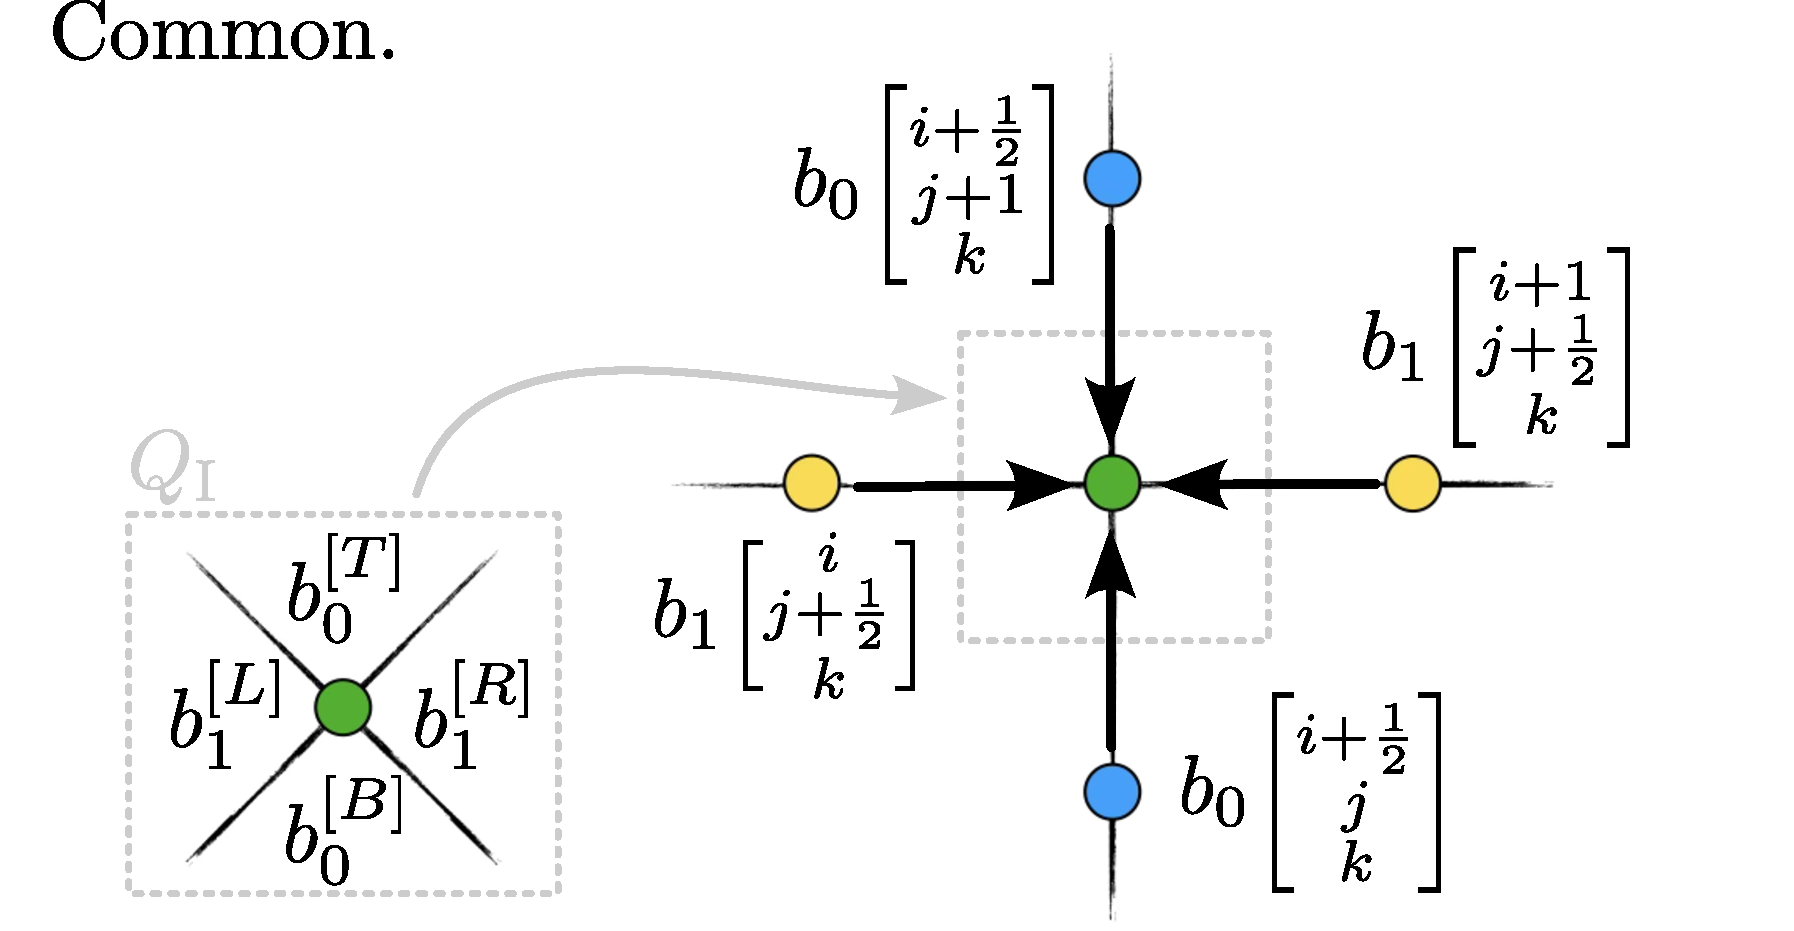
\includegraphics[width=0.65\linewidth]{figures/quokka-mhd/schematics/b-common.pdf}
    \caption{Schematic representation of the magnetic field reconstruction step, which is common to all our EMF reconstruction schemes. In this step, face-centred magnetic fields are interpolated to cell corners. In the example shown above, the face-centred magnetic field component $b_1$, stored at the $x_1$ cell faces (blue points), is interpolated to the cell edge (red point), yielding magnetic field components $b_1^{\{B\}}$ and $b_1^{\{T\}}$ at the bottom and top of the edge. Similarly, component $b_2$, stored at $x_2$ cell faces (green points), is interpolated to the cell edge to yield $b_2^{\{L\}}$ and $b_2^{\{R\}}$, values on the left and right side of the edge.}
    \label{fig:schematic:b-common}
\end{figure}

All of the schemes start in the same way, which we illustrate in \autoref{fig:schematic:b-common}. We first reconstruct the face-centred magnetic field component $b_1\EvalAtH{i \pm 1/2}{j}{k}$ in the $x_2$- direction to yield $b_{1}^{\cbrac{S_\mathrm{II}}}\EvalAtH{i \pm 1/2}{j \pm 1/2}{k}$, and reconstruct the face-centred magnetic field component $b_2\EvalAtH{i}{j \pm 1/2}{k}$ in the $x_1$-direction to yield $b_{2}^{\cbrac{S_\mathrm{I}}}\EvalAtH{i \pm 1/2}{j \pm 1/2}{k}$. Here the subscripts $L$ or $R$ indicate values on the left and right side of an $x_1$-face, and similarly the subscripts $B$ and $T$ indicate the values on the bottom and top of a $x_2$-face.\footnote{
    Formally there is of course no difference between ``left'' and ``bottom'', or between ``right'' and ``top'', but we use different terminology to help make clear whether we are discussing an interface oriented in the $x_1$-direction, which uses left and right, and one in the $x_2$-direction, which uses top and bottom.
} The $L$ and $R$ values, and the $B$ and $T$ values, may be different due to limiting in the reconstruction. This reconstruction, and all the other reconstruction steps we will describe below, can be done using any of the PC, PLM, PPM, or PPM-EP interpolators described in \autoref{sec:methods:flux} -- the choices of reconstruction scheme and interpolator are independent. Below in \autoref{sec:performance} we will test multiple combinations of interpolator and reconstruction scheme.

Once the magnetic fields are reconstructed to the cell edges, the remaining steps differ depending on the scheme.

\begin{figure}
    \centering
    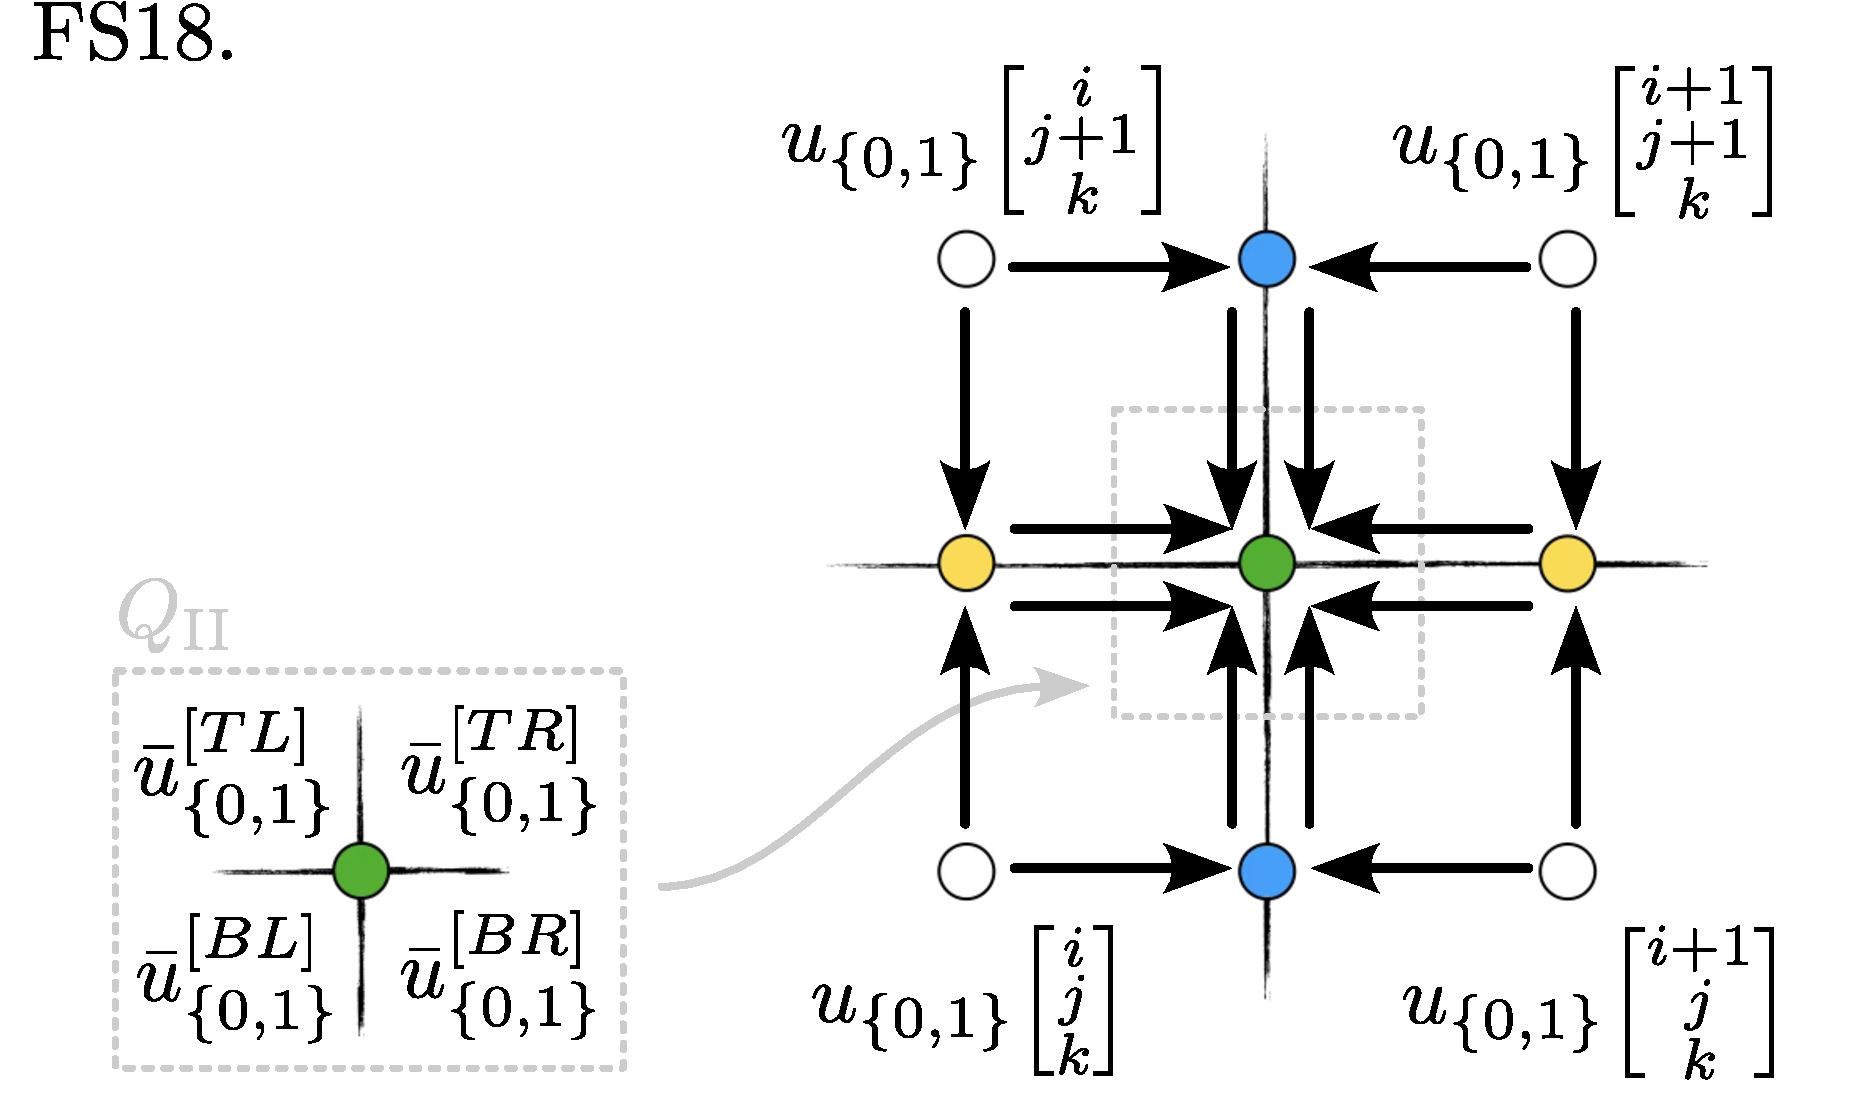
\includegraphics[width=0.65\linewidth]{figures/quokka-mhd/schematics/u-fs18.pdf}
    \caption{Schematic representation of the velocity interpolation part of the \citetalias{Felker18a} EMF reconstruction scheme. In this scheme, the velocity components $u_1$ and $u_2$ stored at cell centres (black points) are interpolated to the edge (red point) in two steps -- first by interpolating to the cell faces in the $x_1$ and $x_2$ directions (blue and green points), then by interpolating in the $x_2$ and $x_1$ directions to reach the cell edge, yielding two estimates of the velocity at the edge. The two estimates are then averaged to yield $\bar{u}_{1,2}$. This process occurs in each of the four corners adjacent to the edge, yielding four values $\bar{u}_{1,2}^{Q_\mathrm{II}}$ at the cell edge. These four velocity estimates are combined with the two magnetic field estimates (\autoref{fig:schematic:b-common}) to yield the EMF at the cell edge (\autoref{eqn:emf:fs18}).}
    \label{fig:schematic:fs18}
\end{figure}

\paragraph{The \citet[hereafter \citetalias{Felker18a}]{Felker18a} strategy.}
This strategy is illustrated in \autoref{fig:schematic:fs18}. We begin from the cell-centred velocity $\mVector{u}\EvalAtH{i}{j}{k}$ and reconstruct to the cell faces where the magnetic fields are stored, then reconstruct to the cell edges where they are required to compute the EMF. Quantitatively the steps are:
\begin{enumerate}
    \item Reconstruct cell-centred velocities to cell faces. We reconstruct $\mVector{u}\EvalAtH{i}{j}{k}$ in the $x_1$- and $x_2$-directions to obtain $\mVector{u}^{\cbrac{S_\mathrm{I}: x_1}}\EvalAtH{i \pm 1/2}{j}{k}$ and $\mVector{u}^{\cbrac{S_\mathrm{II}: x_2}}\EvalAtH{i}{j \pm 1/2}{k}$, where the superscript $x_1$ or $x_2$ indicates the direction in which reconstruction was performed.\footnote{
        Note that only the 1- and 2-components of $\mVector{u}$ are needed, but for notational simplicity we describe the procedure as acting on the full vector $\mVector{u}$. Our code implementation only acts on the two components that are needed.
    }
    \item Reconstruct face-centred velocities to cell edges. We reconstruct the $x_1$-face-centred velocities in the $x_2$-direction, and the $x_2$-face-centred velocities in the $x_1$-direction. This yields eight quantities at each edge, which we denote $\mVector{u}^{\cbrac{Q_\mathrm{II}: x_1 x_2}}\EvalAtH{i \pm 1/2}{j \pm 1/2}{k}$ and $\mVector{u}^{\cbrac{Q_\mathrm{II}: x_2 x_1}}\EvalAtH{i \pm 1/2}{j \pm 1/2}{k}$. Here the four possible subscripts $LB$, $RB$, $LT$, and $RT$, indicate the four possible corners adjacent to the edge, while the superscripts $x_1 x_2$ and $x_2 x_1$ indicate the reconstruction order, with $x_1 x_2$ indicating a quantity that was produced by reconstructing first in the $x_1$-direction to reach the $x_1$-face and then in the $x_2$-direction, and $x_2 x_1$ indicating the opposite order. Note that reconstruction is not a commutative operation, so these two possible orderings in general yield distinct values.
    \item Average over reconstruction orderings. The previous step produces two estimates for each of the four corner quantities $LB$, $RB$, $LT$, and $RT$ -- one produced by reconstructing in $x_1$ then $x_2$, and one produced by reconstructing in the opposite order. We now average those two estimates, computing
    \begin{align*}
        \bar{\mVector{u}}^{\cbrac{Q_\mathrm{II}}}\EvalAtH{i \pm 1/2}{j \pm 1/2}{k}
            &= \frac{1}{2} \Big(
                \mVector{u}^{\cbrac{Q_\mathrm{II}: x_1 x_2}}\EvalAtH{i \pm 1/2}{j \pm 1/2}{k}
            \\
            &\nquad[4]
                + \mVector{u}^{\cbrac{Q_\mathrm{II}: x_2 x_1}}\EvalAtH{i \pm 1/2}{j \pm 1/2}{k}
            \Big)
        .
    \end{align*}
    This reduces the number of distinct estimates of $\mVector{u}$ at each cell edge from eight to four.
    \item Compute the EMFs at the edges. We now have four velocity estimates and two magnetic field estimates at each edge. The final step is to combine these to produce four EMF estimates at each edge:
\begin{align}
    &\varepsilon_{3}^{\{Q_\mathrm{II}\}}\EvalAtH{i \pm 1/2}{j \pm 1/2}{k}
        = -\bar{u}_{1}^{\{Q_\mathrm{II}\}}\EvalAtH{i \pm 1/2}{j \pm 1/2}{k}
            b_{2}^{\cbrac{S_\mathrm{I}}}\EvalAtH{i \pm 1/2}{j \pm 1/2}{k}
        \nonumber \\
        &\nquad[5] + \bar{u}_{2}^{\{Q_\mathrm{II}\}}\EvalAtH{i \pm 1/2}{j \pm 1/2}{k}
            b_{1}^{\cbrac{S_\mathrm{II}}}\EvalAtH{i \pm 1/2}{j \pm 1/2}{k}
    , \label{eqn:emf:fs18}
\end{align}
where $S_\mathrm{I}$ can be either $L$ or $R$, and $S_\mathrm{II}$ can be either $B$ or $T$. These represent four estimates of the EMF, which we will combine using one of the averaging methods described in \autoref{sec:methods:emf:averaging}.
\end{enumerate}

\begin{figure}
    \centering
    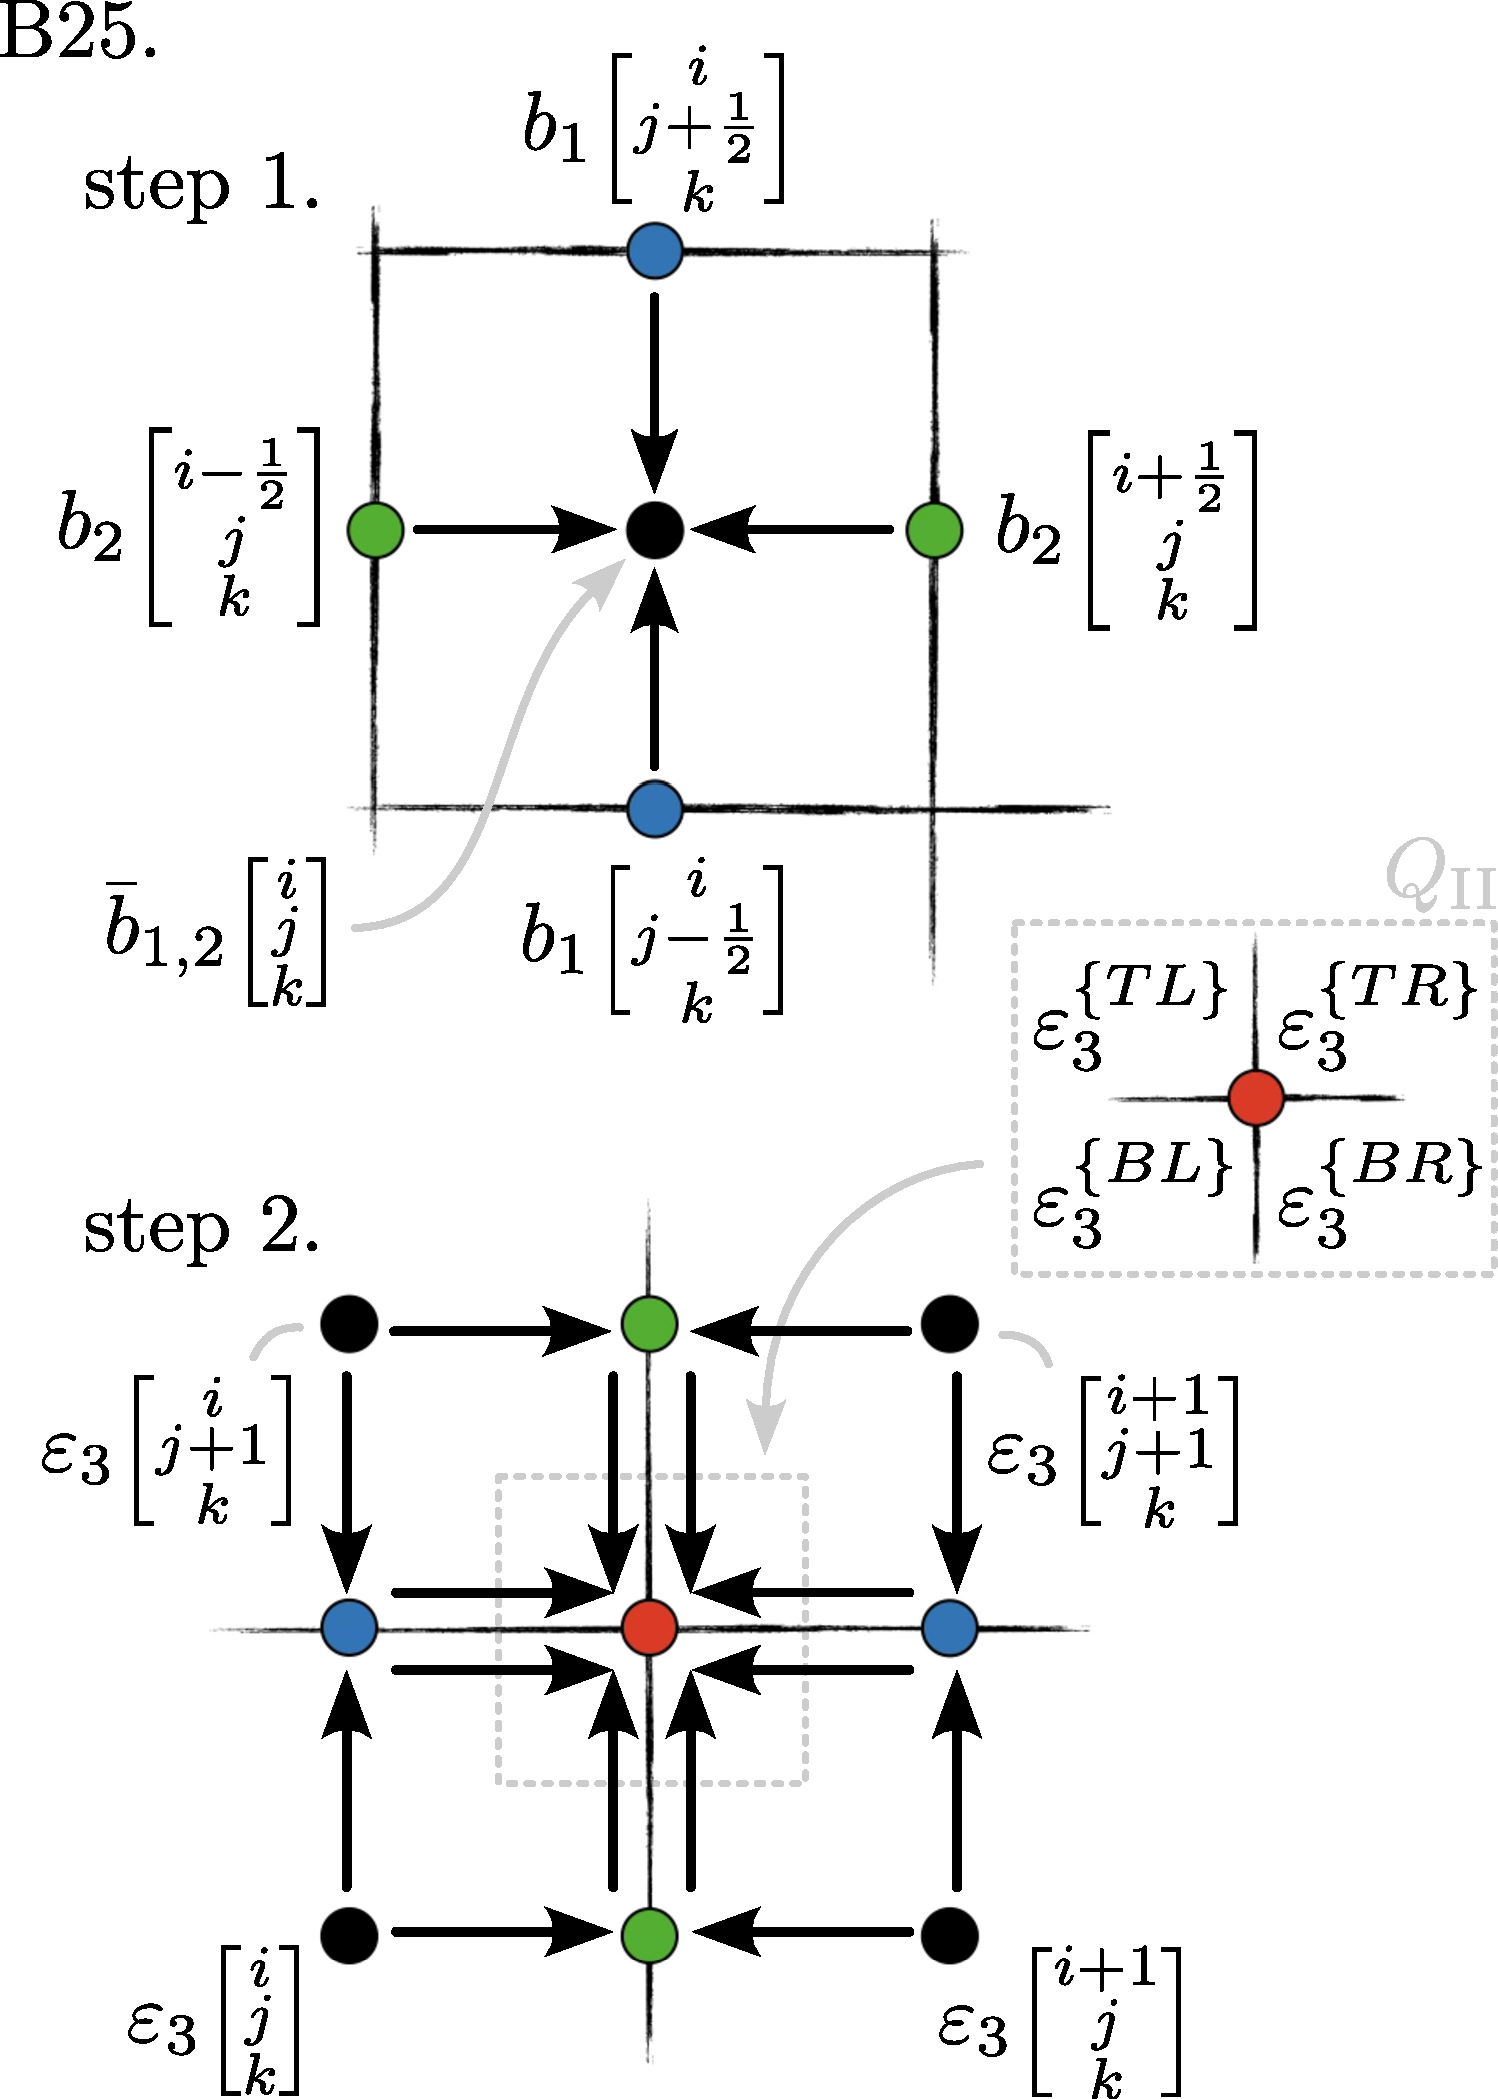
\includegraphics[width=0.65\linewidth]{figures/quokka-mhd/schematics/B25.pdf}
    \caption{Schematic representation of the \citetalias{Balsara25a} EMF reconstruction scheme. In the first step, the magnetic field components $b_1$ and $b_2$ stored at the $x_1$ and $x_2$ cell faces (green and blue points) are averaged to the cell centre (black point), yielding mean magnetic fields $\bar{b}_{1,2}$ there. These are then combined with the cell centre velocity to get a cell-centre EMF component $\epsilon_3$. In the second step, this EMF component is interpolated to the cell edge (red point) in two steps -- it is first interpolated in the $x_1$ and $x_2$ directions to the cell faces (blue and green points), then in the $x_2$ and $x_1$ directions to the cell edge. The two interpolation orderings are averaged to produce mean EMF $\bar{\epsilon}_3$. This procedure happens in all four corners of the cell, yielding four EMF estimates $\bar{\varepsilon}_3^{Q_\mathrm{II}}$}
    \label{fig:schematic:b25}
\end{figure}

\paragraph{The \citet[hereafter \citetalias{Balsara25a}]{Balsara25a} strategy.}
In this strategy, which is illustrated in \autoref{fig:schematic:b25}, we first average the face-centred magnetic fields to the cell centre, compute the EMFs from the cell-centred velocities and magnetic fields, and then interpolate the EMFs to the cell edges. In detail, the steps are:
\begin{enumerate}
    \item Average the face-centred magnetic fields to cell centres. Thus we compute
    \begin{align*}
        b_1\EvalAtH{i}{j}{k}
            = \frac{1}{2} \Big(
                    b_1\EvalAtH{i + 1/2}{j}{k}
                        + b_1\EvalAtH{i - 1/2}{j}{k}
                \Big)
    \end{align*}
    and similarly for $b_2\EvalAtH{i}{j}{k}$.
    \item Evaluate the $x_3$-component of the cell-centred EMF as
    \begin{align*}
        \varepsilon_3\EvalAtH{i}{j}{k}
            = -u_1\EvalAtH{i}{j}{k} b_2\EvalAtH{i}{j}{k}
                + u_2\EvalAtH{i}{j}{k} b_1\EvalAtH{i}{j}{k}
        .
    \end{align*}
    \item Reconstruct the cell-centred EMFs to the cell faces. This yields $\varepsilon_{3}^{\cbrac{S_\mathrm{I}: x_1}}\EvalAtH{i \pm 1/2}{j}{k}$, $\varepsilon_{3}^{\cbrac{S_\mathrm{II}: x_2}}\EvalAtH{i}{j \pm 1/2}{k}$, where as in the \citetalias{Felker18a} method the subscripts $L$ and $R$ indicate the reconstructed quantities on the left and right side of an $x_1$-face, $B$ and $T$ indicate the bottom and top of a $x_2$-face, and the superscripts $x_1$ and $x_2$ indicate the direction of reconstruction used to produce that quantity.
    \item Reconstruct the face-centred EMFs to cell edges. In this step we reconstruct the $x_1$-face-centred EMF in the $x_2$-direction and the $x_2$-face-centred EMF in the $x_1$ direction. This yields eight estimates of each EMF at the edge, which we denote $\varepsilon_{3}^{\cbrac{Q_\mathrm{II}: x_1 x_2}}\EvalAtH{i \pm 1/2}{j \pm 1/2}{k}$ and $\varepsilon_{3}^{\cbrac{Q_\mathrm{II}: x_2 x_1}}\EvalAtH{i \pm 1/2}{j \pm 1/2}{k}$, where the superscripts $x_1 x_2$ and $x_2 x_1$ indicate whether we reconstructed first in the $x_1$ and then the $x_2$ direction, or the reverse.
    \item Average over reconstruction orderings. As in the \citetalias{Felker18a} method, we have two estimates for each of the four corners LB, RB, LT, and RT, resulting from the two possible orderings of the one-dimensional reconstructions. We now average these two orderings, yielding $\varepsilon_{3}^{\cbrac{Q_\mathrm{II}}}\EvalAtH{i \pm 1/2}{j \pm 1/2}{k} = (\varepsilon_{3}^{\cbrac{Q_\mathrm{II}: x_1 x_2}}\EvalAtH{i \pm 1/2}{j \pm 1/2}{k} + \varepsilon_{3}^{\cbrac{Q_\mathrm{II}: x_2 x_1}}\EvalAtH{i \pm 1/2}{j \pm 1/2}{k})/2$. This leaves the four final EMF estimates at the edge that we will combine using one of the averaging methods from \autoref{sec:methods:emf:averaging}.    
\end{enumerate}
    
Note that in the \citetalias{Balsara25a} reconstruction scheme does not directly make use of the face-centred magnetic fields reconstructed to the cell edges, which we compute as a first step in all reconstruction schemes. However, since these reconstructed magnetic fields are required for both the EMF averaging schemes described in \autoref{sec:methods:emf:averaging}, we carry out this step anyway.

\begin{figure}
    \centering
    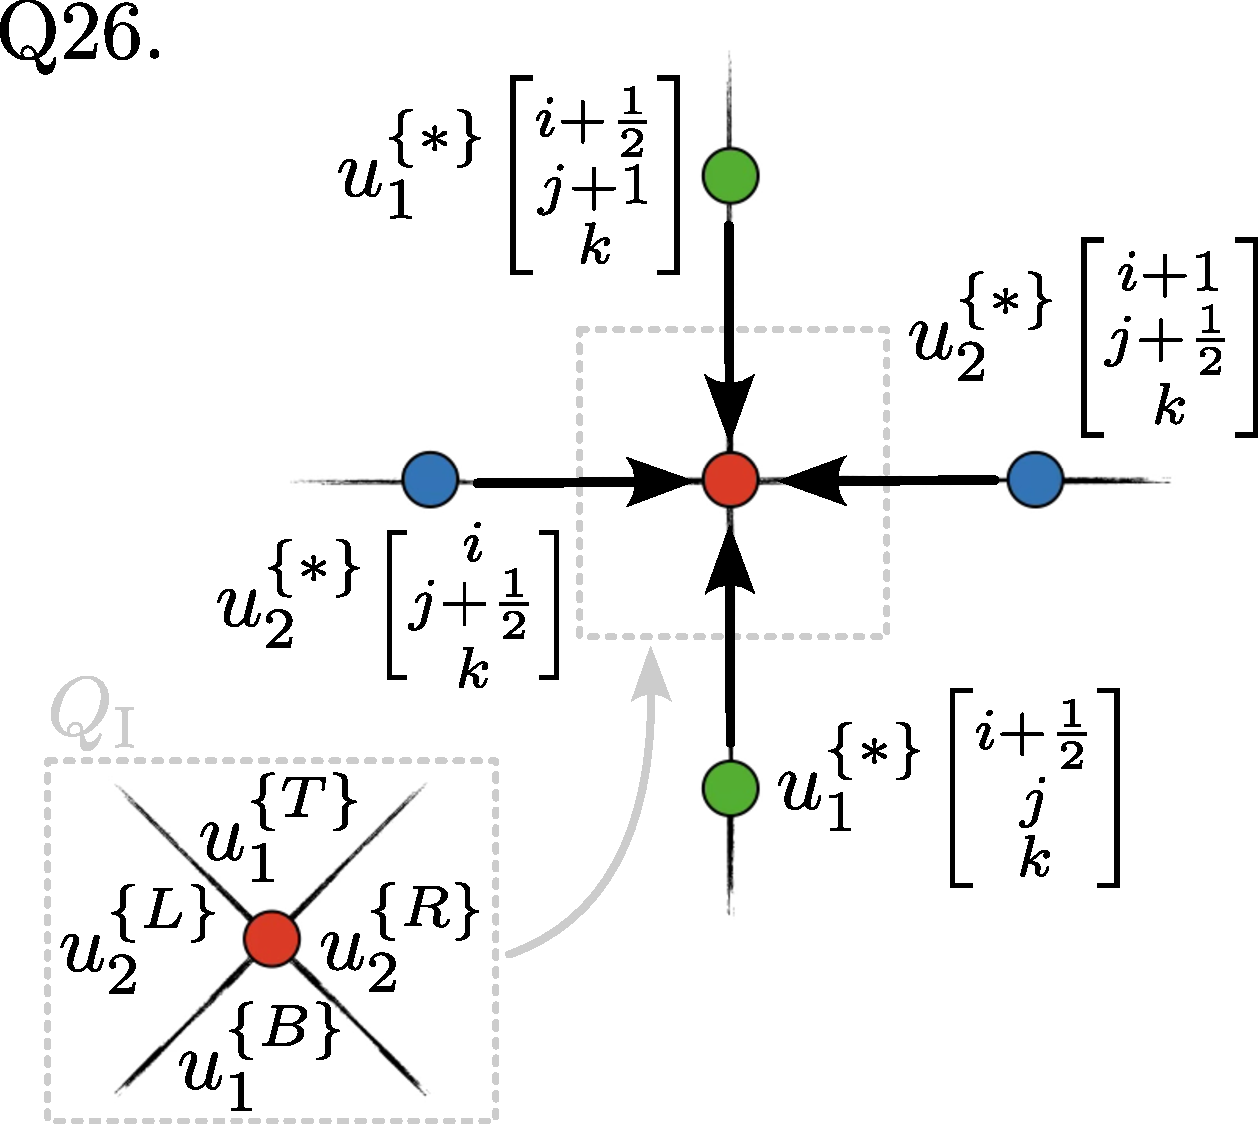
\includegraphics[width=0.6\linewidth]{figures/quokka-mhd/schematics/u-Q26.pdf}
    \caption{Schematic representation of the velocity interpolation part of the Q26 EMF reconstruction scheme. The scheme starts from the face velocities derived from the Riemann solver mass flux and upwind density, which we denote $u_1^{\cbrac{*}}$ and $u_2^{\cbrac{*}}$, at the $x_1$ and $x_2$ cell faces (blue and green points). These are then interpolated to the cell edge (red point), yielding estimates $u_1^{\{B\}}$ and $u_1^{\{T\}}$ for the velocity in the $x_1$ direction, and $u_2^{\{L\}}$ and $u_2^{\{R\}}$ for the velocity in the $x_2$ direction. These are then combined with the interpolated magnetic fields (\autoref{fig:schematic:b-common} to yield an estimate of the cell edge EMF (\autoref{eqn:emf:q26}).}
    \label{fig:schematic:q26}
\end{figure}
    
\paragraph{The Quokka 2026 (Q26) strategy.} The final strategy that we consider, illustrated in \autoref{fig:schematic:q26}, is new, though it is similar in spirit to an approach taken by \citet{Mignone21a}. As with the \citetalias{Felker18a} method, we bring the velocity and magnetic field to the cell edge separately and combine them there to compute the EMF, but with an important difference: rather than reconstructing velocities from the cell centre to the face and then from the face to the edge, we instead begin from face velocities obtained directly from the Riemann solver (\autoref{sec:methods:flux}). Specifically, we obtain a  velocity at each face by dividing the mass flux returned by the Riemann solver by the left or right state density, depending on which is the upwind direction at that face. We denote the velocities on the $x_1$- and $x_2$-faces derived via this procedure as $u_{1}^{\cbrac{*}}\EvalAtH{i \pm 1/2}{j}{k}$ and $u_{2}^{\cbrac{*}}\EvalAtH{i}{j \pm 1/2}{k}$. This means that we start will all the quantities required to compute the EMF already stored at cell faces, and we require only a single reconstruction to reach cell edges. The steps in detail are:
\begin{enumerate}
    \item Reconstruct the face velocities to cell edges. We reconstruct $u_{1}^{\cbrac{*}}$ in the $x_2$-direction to yield $u_{1}^{\cbrac{*;S_\mathrm{II}}}\EvalAtH{i \pm 1/2}{j \pm 1/2}{k}$, and reconstruct $u_{2}^{\cbrac{*}}$ in the $x_1$-direction to yield $u_{2}^{\cbrac{*;S_\mathrm{I}}}\EvalAtH{i \pm 1/2}{j \pm 1/2}{k}$. As previously, $L$, $R$, $T$, and $B$ indicate states on the left, right, top, and bottom of the edge.
    \item Compute the EMFs at the edges. For the $x_2$ edges, we can compute four estimates of the EMF as:
\begin{align}
    &\varepsilon_{3}^{\{Q_\mathrm{II}\}}\EvalAtH{i \pm 1/2}{j \pm 1/2}{k}
        = -u_{1}^{\cbrac{*;S_\mathrm{II}}}\EvalAtH{i \pm 1/2}{j \pm 1/2}{k}
            b_{2}^{\cbrac{S_\mathrm{I}}}\EvalAtH{i \pm 1/2}{j \pm 1/2}{k} 
        \nonumber \\
        &\nquad[7] + u_{2}^{\cbrac{*;S_\mathrm{I}}}\EvalAtH{i \pm 1/2}{j \pm 1/2}{k}
            b_{1}^{\cbrac{S_\mathrm{II}}}\EvalAtH{i \pm 1/2}{j \pm 1/2}{k}
    , \label{eqn:emf:q26}
\end{align}
where $S_\mathrm{I}$ can be either $L$ or $R$, and $S_\mathrm{II}$ can be either $B$ or $T$. These are the four quadrant estimates on which our EMF averaging scheme will act.
\end{enumerate}

In comparison to the \citetalias{Felker18a} and \citetalias{Balsara25a} schemes, it is clear that the Q26 scheme involves significantly fewer reconstructions and fewer temporary variables. However, this is partially offset by an increase in the cost of the flux calculation associated with ghost zones. For reasons we discuss in \autoref{sec:methods:emf:averaging}, our EMF averaging schemes require that we calculate the fluxes not just in the real cells of the domain, but for one ghost cell. The Q26 scheme in general requires more, at least if we wish to use a higher-order reconstruction method: we must be able to reconstruct $u_{1}^{\cbrac{*}}$ in the $x_2$-direction, which requires knowledge of the star state not just at the one ghost face adjacent to the real cells, but in two ghost zones for PLM interpolation, and three for PPM or PPM-EP. We are therefore required to solve the Riemann problem in this many more ghost zones. We will test the performance impact of this trade-off -- fewer reconstruction steps but more ghost zones -- in \autoref{sec:performance}.

\subsubsection{The EMF averaging scheme}
\label{sec:methods:emf:averaging}

Each of the reconstruction schemes described in \autoref{sec:methods:emf:reconstruction} yields estimates of the EMF around each corner of the cell edge; for the $x_3$-edges, these are denoted $\varepsilon_{3}^{\{Q_\mathrm{II}\}}\EvalAtH{i \pm 1/2}{j \pm 1/2}{k}$. The final step is to average these together to yield a single estimate of the EMF, $\varepsilon_{3}\EvalAtH{i \pm 1/2}{j \pm 1/2}{k}$. We consider two schemes for doing so below. In addition to the EMFs, these schemes make use of the magnetic fields reconstructed to the cell edges, $b_{1}^{\cbrac{S_\mathrm{II}}}\EvalAtH{i \pm 1/2}{j \pm 1/2}{k}$ and $b_{2}^{\cbrac{S_\mathrm{I}}}\EvalAtH{i \pm 1/2}{j \pm 1/2}{k}$, and the minimum and maximum wavespeeds on the four faces adjacent to the edge as computed during the flux update. We denote these wavespeeds $\alpha_{1,2}^{\cbrac{\pm}}$, where $x_1$ or $x_2$ indicates the direction of the face across which the speed is calculated, and $\pm$ indicates the minimum (most negative) or maximum wavespeed. We compute $\alpha_{1,2}^{\cbrac{\pm}}$ following the procedure outlined in Appendix A of \citetalias{Felker18a}. Note that computing these wavespeeds requires that we solve the Riemann problem not just over the real cells of the domain, but for one ghost cell as well.

\paragraph{The \citet[hereafter \citetalias{Londrillo04a}]{Londrillo04a} strategy.}
Our first option combines the four corner EMFs using the solution to a 2D HLL Riemann solver, following the approach developed by \citetalias{Londrillo04a}. Our exact implementation of this solution is given by equation 41 of \citetalias{Felker18a}. This yields a single upwinded EMF estimate $\varepsilon_3\EvalAtH{i \pm 1/2}{j \pm 1/2}{k}$ at each cell edge.

\paragraph{The \citet[hereafter \citetalias{Balsara25b}]{Balsara25b} strategy.} 
Our second option uses a new 2D Riemann solver developed by \citetalias{Balsara25b} to combine the EMFs. The implementation of this Riemann solver that we follow is given by equation 3.10 of \citetalias{Balsara25a}. Note that although both this Riemann solver method and the interpolation scheme we have described as the \citetalias{Balsara25a} strategy were introduced together, they are independent in the sense that we can apply the \citetalias{Balsara25b} Riemann solver to any combination of four corner EMFs regardless of the reconstruction scheme used to obtain them, and, conversely, we are free to use the  \citetalias{Londrillo04a} rather than the \citetalias{Balsara25b} averaging strategy on the corner EMFs even if they were derived using the \citetalias{Balsara25a} reconstruction method. Below in \autoref{sec:performance} we will in fact test multiple such combinations.

\subsection{Time stepping with flux correction}
\label{sec:methods:time-stepping}

Now that we have describe our method for compute the fluxes through faces and the EMFs around cell edges, we are in a position to describe an overall time stepping scheme. As discussed in \citetalias{Wibking22a}, by default \textsc{Quokka} uses RK2-SSP\footnote{
    In problems that include the radiation submodule, we change to asymptotic-preserving IMEX PD-ARS method following \citet{Chu19a}, implemented as described by \citet{He24a}. However, this method reduces to RK2-SSP for the non-radiation parts of the update, including MHD, and we therefore will not bother to distinguish the two schemes here.
} time stepping \citep{Shu88a}. However, even for time steps that obey the CFL condition, this method can become unstable for extreme problems; indeed, there is no known method for guaranteeing stability in multidimensional schemes with accuracies greater than first order. To mitigate this problem, we introduce a modified time stepping strategy featuring a method for first order flux correction (FOFC) that maintains stability even in difficult-to-integrate flows.

\begin{figure}
    \centering
    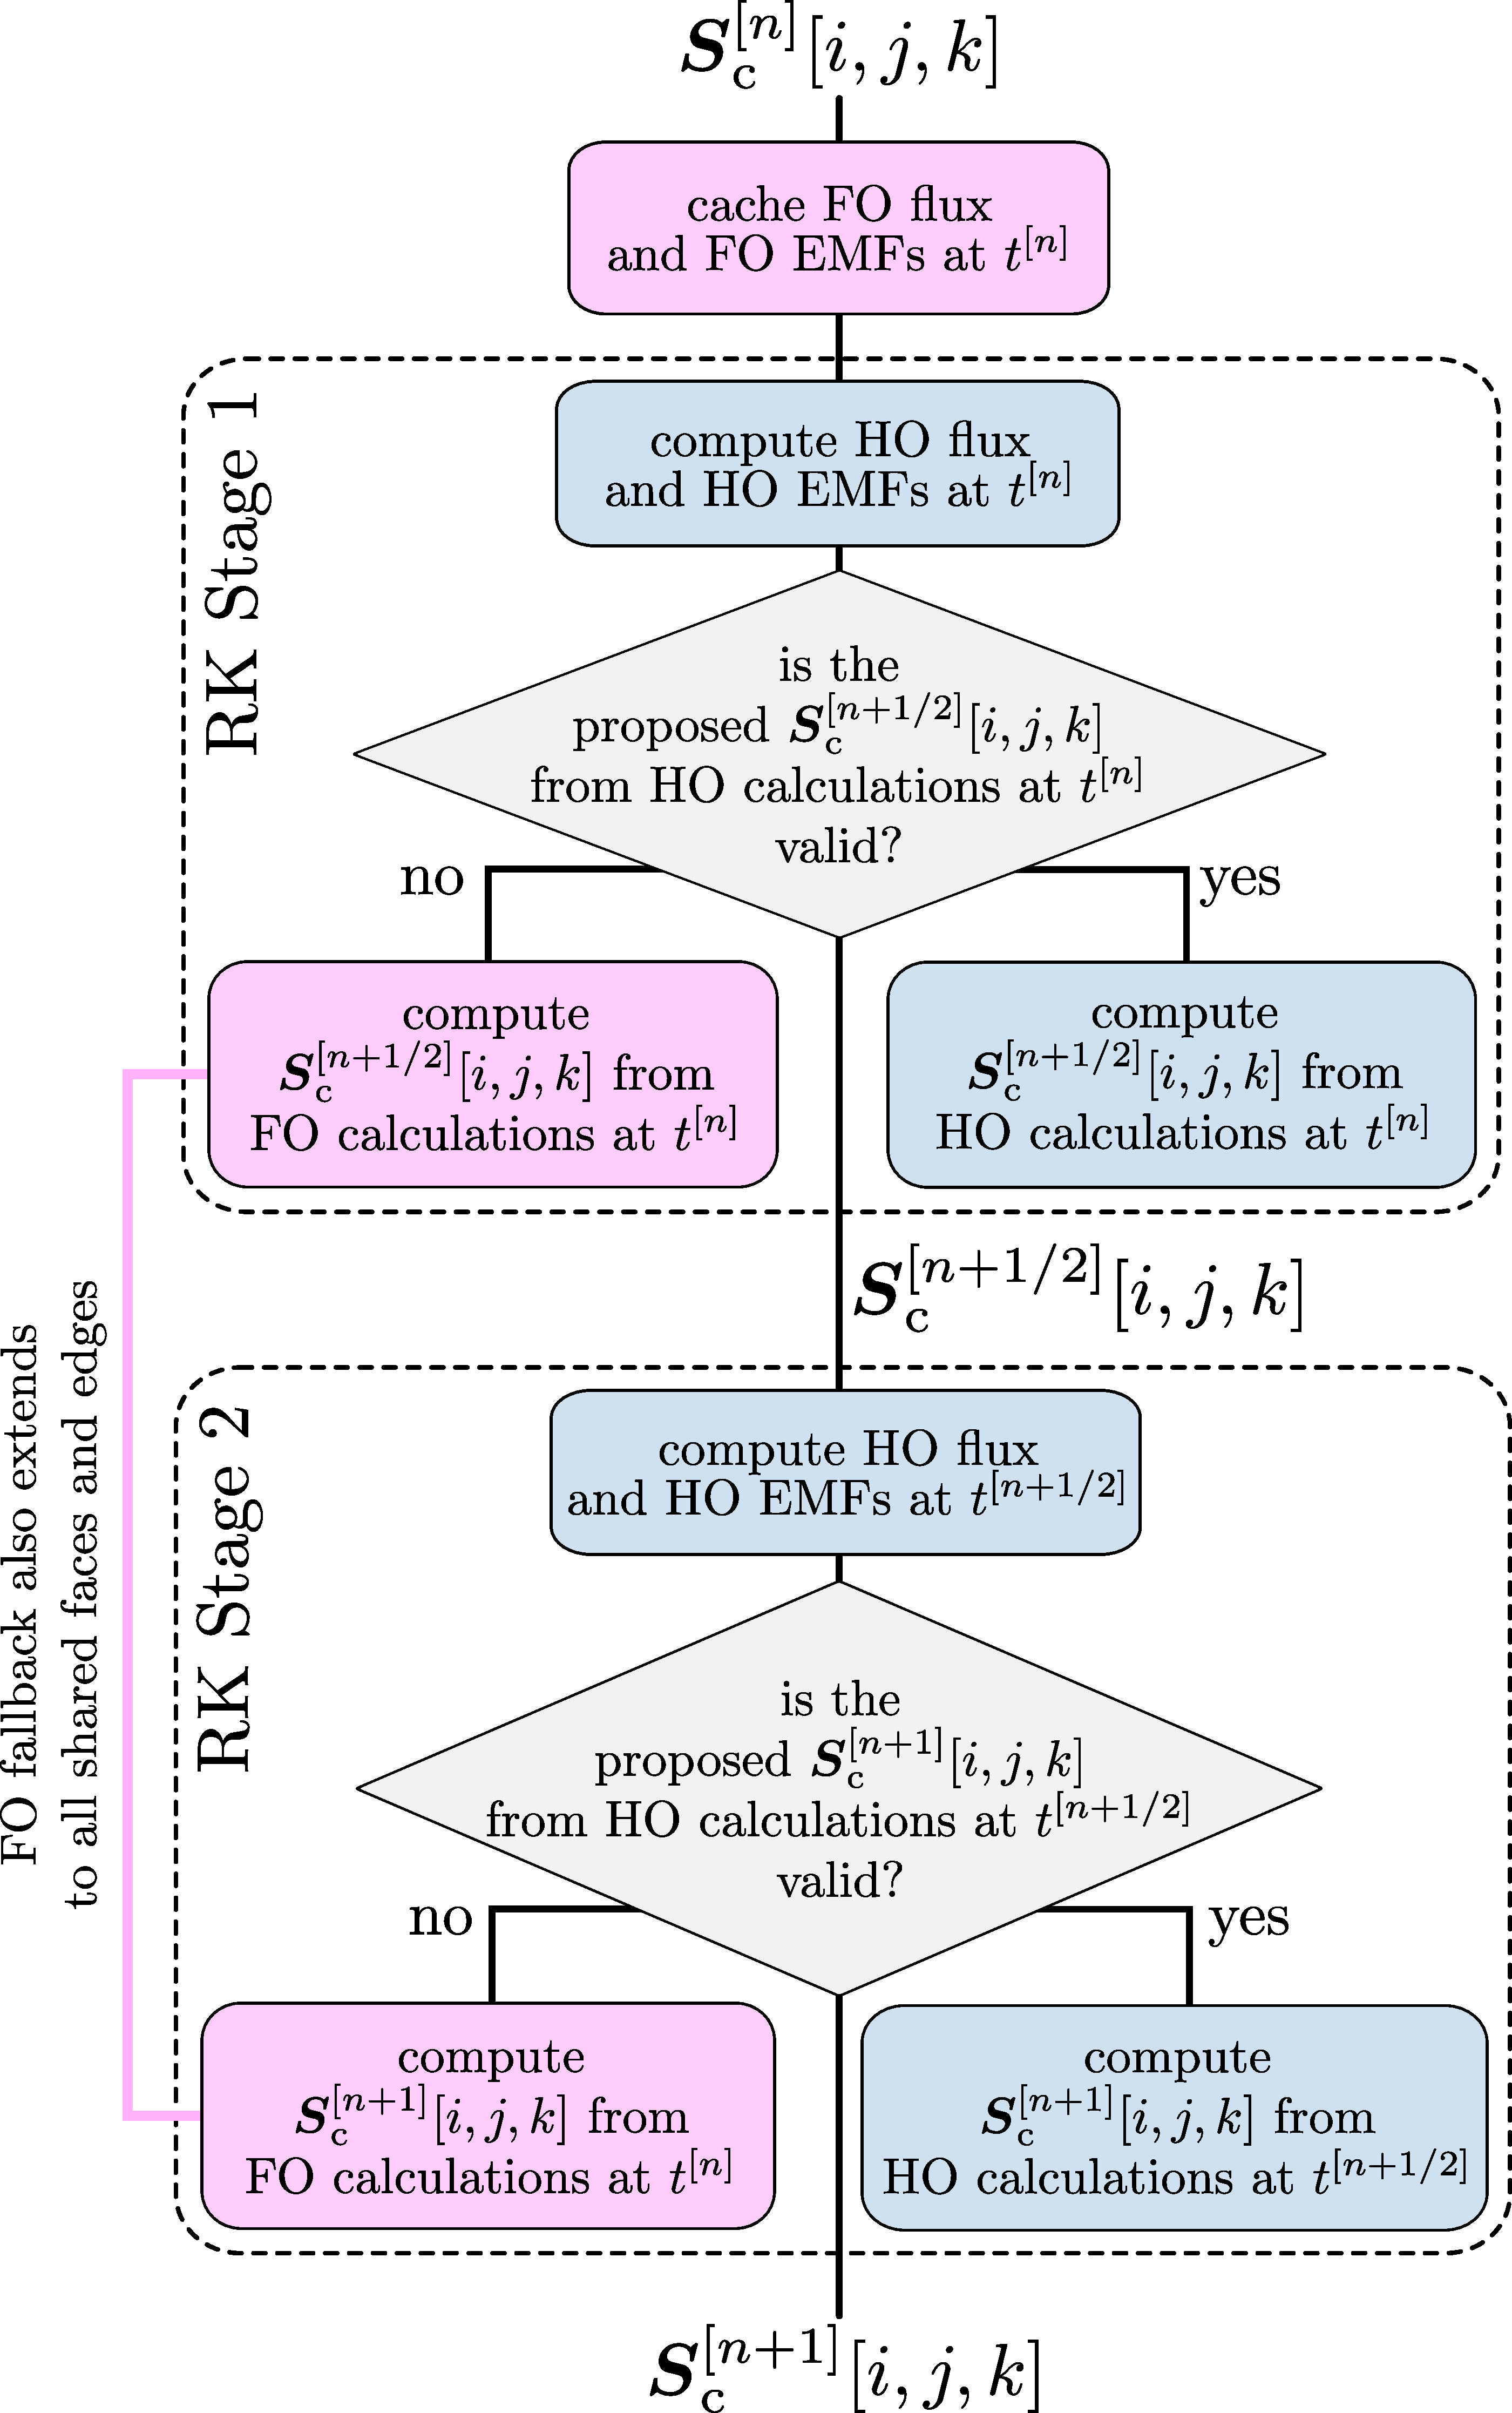
\includegraphics[width=0.7\linewidth]{figures/quokka-mhd/schematics/flowchart.pdf}
    \caption{Flow chart of the \textsc{Quokka} time stepping strategy combining RK2-SSP with first order flux correction. Here quantities labelled as high-order (HO) are computed using either PLM, PPM, or PPM-EP interpolation and the HLLD Riemann solver, while those labelled first-order (FO) are computed using PC interpolation and the LLF Riemann solver.}
    \label{fig:schematic:flowchart}
\end{figure}

We summarise the steps in our time stepping strategy in \autoref{fig:schematic:flowchart}. We start at time $t^{[n]}$ with a set of cell-centred conserved quantities $\mVector{S}_\mathrm{c}^{[n]}\EvalAtH{i}{j}{k}$ and face-centred magnetic fields $b_1^{[n]}\EvalAtH{i + 1/2}{j}{k}$, and similarly for $b_2$ and $b_3$. The steps are carry out to advance to time $t^{[n + 1]} = t^{[n]} + \Delta t$ are:\footnote{
    For simplicity we omit the extra steps involved if we are using \textsc{Quokka}'s dual energy formalism. If dual energy is in use, we apply the dual energy correction following each calculation of a cell-centred state \citep{Wibking22a}.
}
\begin{enumerate}
    \item First compute a set of first-order, highly-dissipative fluxes of conserved cell-centred quantities and EMFs at each cell face and edge using the old-time state $\mVector{S}_\mathrm{c}^{[n]}\EvalAtH{i}{j}{k}$ and $b_1^{[n]}\EvalAtH{i + 1/2}{j}{k}$. We carry out the flux computation as described in \autoref{sec:methods:flux}, using PC interpolation and the LLF Riemann solver, and then we use the resulting wavespeeds (and for the Q26 method star states) to compute the EMFs as described in \autoref{sec:methods:emf}. We denote the first-order fluxes of conserved cell-centred quantities that result from this procedure as $\mVector{F}_\mathrm{FO}^{[n]}\EvalAtH{i \pm 1/2}{j}{k}$ and the corresponding EMFs as $\mVector{\varepsilon}_\mathrm{FO}^{[n]}\EvalAtH{i \pm 1/2}{j \pm 1/2}{k}$, and similarly for faces and edges in other directions.
    \label{step:fo:cache}
    \item First RK stage:
        \begin{enumerate}
            \item Compute a set of high-order, low-dissipation fluxes and EMFs as described in \autoref{sec:methods:flux} and \autoref{sec:methods:emf}. This calculation is identical to that in \autoref{step:fo:cache} except that we use a higher-order interpolation scheme (PLM, PPM, or PPM-EP as specified by the user) and the HLLD Riemann solver rather than PC and LLF. We denote the resulting fluxes and EMFs as $\mVector{F}_\mathrm{HO}^{[n]}\EvalAtH{i \pm 1/2}{j}{k}$ and $\mVector{\varepsilon}_\mathrm{HO}^{[n]}\EvalAtH{i \pm 1/2}{j \pm 1/2}{k}$.
            \label{step:rk1:ho}
            \item Compute a proposed intermediate set of conserved cell-centred conserved quantities and face-centred magnetic fields as
            \begin{align}
                &\mVector{S}_\mathrm{c}^{[n + 1/2]}\EvalAtH{i}{j}{k}
                    = \mVector{S}_\mathrm{c}^{[n]}\EvalAtH{i}{j}{k}
                        + \frac{\Delta t}{\Delta{x_1}\, \Delta{x_2}\, \Delta{x_3}} \Bigg(
                    \nonumber \\
                    &\nquad[2] \, \Delta{x_2} \, \Delta{x_3} \rbrac{
                            \mVector{F}^{[n]}\EvalAtH{i - 1/2}{j}{k}
                            - \mVector{F}^{[n]}\EvalAtH{i + 1/2}{j}{k}
                        }
                    \nonumber \\
                    &\nquad[1] + \Delta{x_1} \, \Delta{x_3} \rbrac{
                            \mVector{F}^{[n]}\EvalAtH{i}{j - 1/2}{k}
                            - \mVector{F}^{[n]}\EvalAtH{i}{j + 1/2}{k}
                        }
                    \nonumber \\
                    &\nquad[1] + \Delta{x_1} \, \Delta{x_2} \rbrac{
                            \mVector{F}^{[n]}\EvalAtH{i}{j}{k - 1/2}
                            - \mVector{F}^{[n]}\EvalAtH{i}{j}{k + 1/2}
                        }
                    \Bigg)
                    \nonumber
            \end{align}
            \begin{align}
                &b_1^{[n + 1/2]}\EvalAtH{i + 1/2}{j}{k}
                    = b_1^{[n]}\EvalAtH{i + 1/2}{j}{k}
                        + \frac{\Delta t}{\Delta{x_2} \, \Delta{x_3}} \Bigg(
                    \nonumber \\
                    &\nquad[3] \, \Delta{x_3} \, \varepsilon_3^{[n]}\EvalAtH{i + 1/2}{j - 1/2}{k}
                        + \Delta{x_2} \, \varepsilon_2^{[n]}\EvalAtH{i + 1/2}{j}{k - 1/2}
                    \nonumber \\
                    &\nquad[2] - \Delta{x_3} \, \varepsilon_3^{[n]}\EvalAtH{i + 1/2}{j + 1/2}{k}
                        - \Delta{x_2} \, \varepsilon_2^{[n]}\EvalAtH{i + 1/2}{j}{k + 1/2}
                \Bigg)
                \nonumber
            \end{align}
            \begin{align}
                b_2^{[n + 1/2]}\EvalAtH{i}{j + 1/2}{k}
                    = \cdots
                . \label{eqn:rk1:update}
            \end{align}
            using the HO versions of all fluxes and EMFs.
            \item Check is any of the intermediate states $\mVector{S}_\mathrm{c}^{[n + 1/2]}\EvalAtH{i}{j}{k}$ are physically invalid; at a minimum this means flagging cell centre states with negative densities, total energies, or internal energies, but we can also flag on additional and more stringent criteria, for example velocities that are unphysically large. Any additional flagging is calculation-dependent, and is left as an option for the user.
            \item For any cell $(i, j, k)$ that is flagged as invalid, replace the HO fluxes and EMFs for all of its faces and edges with their FO equivalents as computed in \autoref{step:fo:cache}. Then recompute the cell-centred state and the face-centred magnetic fields for that cell by again applying \autoref{eqn:rk1:update} with the replaced fluxes. This step and the next one are illustrated in \autoref{fig:fofc}.
            \label{step:rk1:fofc}
            \item Also recalculate $\mVector{S}_\mathrm{c}^{[n + 1/2]}\EvalAtH{i}{j}{k}$ and the face-centred magnetic fields for any cell that neighbours a flagged cell; this step ensures that we use consistent fluxes and EMFs for the updates to all cells, a necessary condition for conservation and maintenance of $\nabla\cdot\mVector{b} = 0$.
        \end{enumerate}
    \item Second RK stage:
    \begin{enumerate}
        \item Compute a set of high-order fluxes and EMFs exactly as in \autoref{step:rk1:ho}, but now using the intermediate-time states $\mVector{S}_\mathrm{c}^{[n + 1/2]}\EvalAtH{i}{j}{k}$ and $b_1^{[n + 1/2]}\EvalAtH{i + 1/2}{j}{k}$ as input. We denote these fluxes and EMFs as $\mVector{F}_\mathrm{HO}^{[n + 1/2]}\EvalAtH{i \pm 1/2}{j}{k}$ and $\mVector{\varepsilon}_\mathrm{HO}^{[n + 1/2]}\EvalAtH{i \pm 1/2}{j \pm 1/2}{k}$.
        \item Compute a proposed final set of conserved cell-centred conserved quantities and face-centred magnetic fields as
            \begin{align}
                \mVector{S}_\mathrm{c}^{[n + 1]}\EvalAtH{i}{j}{k}
                    &= \mVector{S}_\mathrm{c}^{[n]}\EvalAtH{i}{j}{k}
                        + \frac{\Delta t}{2 \Delta{x_1}\, \Delta{x_2}\, \Delta{x_3}} \Bigg(
                    \nonumber \\
                    &\nquad[2] \, \Delta{x_2} \, \Delta{x_3} \left(
                                \mVector{F}^{[n]}\EvalAtH{i - 1/2}{j}{k}
                                - \mVector{F}^{[n]}\EvalAtH{i + 1/2}{j}{k}
                            \right)
                    \nonumber \\
                    &\nquad[1] + \Delta{x_1} \, \Delta{x_3} \rbrac{
                                \mVector{F}^{[n]}\EvalAtH{i}{j - 1/2}{k}
                                - \mVector{F}^{[n]}\EvalAtH{i}{j + 1/2}{k}
                            }
                    \nonumber \\
                    &\nquad[1] + \Delta{x_1} \, \Delta{x_2} \rbrac{
                                \mVector{F}^{[n]}\EvalAtH{i}{j}{k - 1/2}
                                - \mVector{F}^{[n]}\EvalAtH{i}{j}{k + 1/2}
                            }
                    \nonumber \\
                    &\nquad[1] + \Delta{x_2} \, \Delta{x_3} \rbrac{
                                \mVector{F}^{[n + 1/2]}\EvalAtH{i - 1/2}{j}{k}
                                - \mVector{F}^{[n + 1/2]}\EvalAtH{i + 1/2}{j}{k}
                            }
                    \nonumber \\
                    &\nquad[1] + \Delta{x_1} \, \Delta{x_3} \rbrac{
                                \mVector{F}^{[n + 1/2]}\EvalAtH{i}{j - 1/2}{k}
                                - \mVector{F}^{[n + 1/2]}\EvalAtH{i}{j + 1/2}{k}
                            }
                    \nonumber \\
                    &\nquad[1] + \Delta{x_1} \, \Delta{x_2} \rbrac{
                                \mVector{F}^{[n + 1/2]}\EvalAtH{i}{j}{k - 1/2}
                                - \mVector{F}^{[n + 1/2]}\EvalAtH{i}{j}{k + 1/2}
                            }
                \Bigg)
                \nonumber
            \end{align}
            \begin{align}
                &b_1^{[n + 1]}\EvalAtH{i + 1/2}{j}{k}
                    = b_1^{[n]}\EvalAtH{i + 1/2}{j}{k}
                        + \frac{\Delta t}{2 \Delta{x_2} \, \Delta{x_3}} \Bigg(
                    \nonumber \\
                    &\nquad[2] \, \Delta{x_3} \, \varepsilon_3^{[n]}\EvalAtH{i + 1/2}{j - 1/2}{k}
                        + \Delta{x_2} \, \varepsilon_2^{[n]}\EvalAtH{i + 1/2}{j}{k - 1/2}
                    \nonumber \\
                    &\nquad[1] - \Delta{x_3} \, \varepsilon_3^{[n]}\EvalAtH{i + 1/2}{j + 1/2}{k}
                        - \Delta{x_2} \, \varepsilon_2^{[n]}\EvalAtH{i + 1/2}{j}{k + 1/2}
                    \nonumber \\
                    &\nquad[1] + \Delta{x_3} \, \varepsilon_3^{[n + 1/2]}\EvalAtH{i + 1/2}{j - 1/2}{k}
                        + \Delta{x_2} \, \varepsilon_2^{[n + 1/2]}\EvalAtH{i + 1/2}{j}{k - 1/2}
                    \nonumber \\
                    &\nquad[1] - \Delta{x_3} \, \varepsilon_3^{[n + 1/2]}\EvalAtH{i + 1/2}{j + 1/2}{k}
                        - \Delta{x_2} \, \varepsilon_2^{[n + 1/2]}\EvalAtH{i + 1/2}{j}{k + 1/2}
                \Bigg)
                \nonumber
            \end{align}
            \begin{align}
                b_2^{[n + 1]}\EvalAtH{i}{j + 1/2}{k}
                    = \cdots
                . \label{eqn:rk2:update}
            \end{align}
        In this calculation we use the fluxes and EMFs at time $[n]$ determined during the first RK stage (HO unless they were replaced during \autoref{step:rk1:fofc}), and we use the HO fluxes at time $[n + 1/2]$.
        \item Again check for physically invalid states $\mVector{S}_\mathrm{c}^{[n + 1]}\EvalAtH{i}{j}{k}$ in any cells. If an invalid state is found, replace the intermediate-time, $[n + 1/2]$, fluxes and EMFs on that cell's faces and edges with the FO ones determined during \autoref{step:fo:cache}, and recompute $\mVector{S}_\mathrm{c}^{[n + 1]}\EvalAtH{i}{j}{k}$ and $b_1^{[n + 1]}\EvalAtH{i + 1/2}{j}{k}$ in both the flagged cell and all its neighbours using the replaced fluxes.
    \end{enumerate}
\end{enumerate}

\begin{figure}
    \centering
    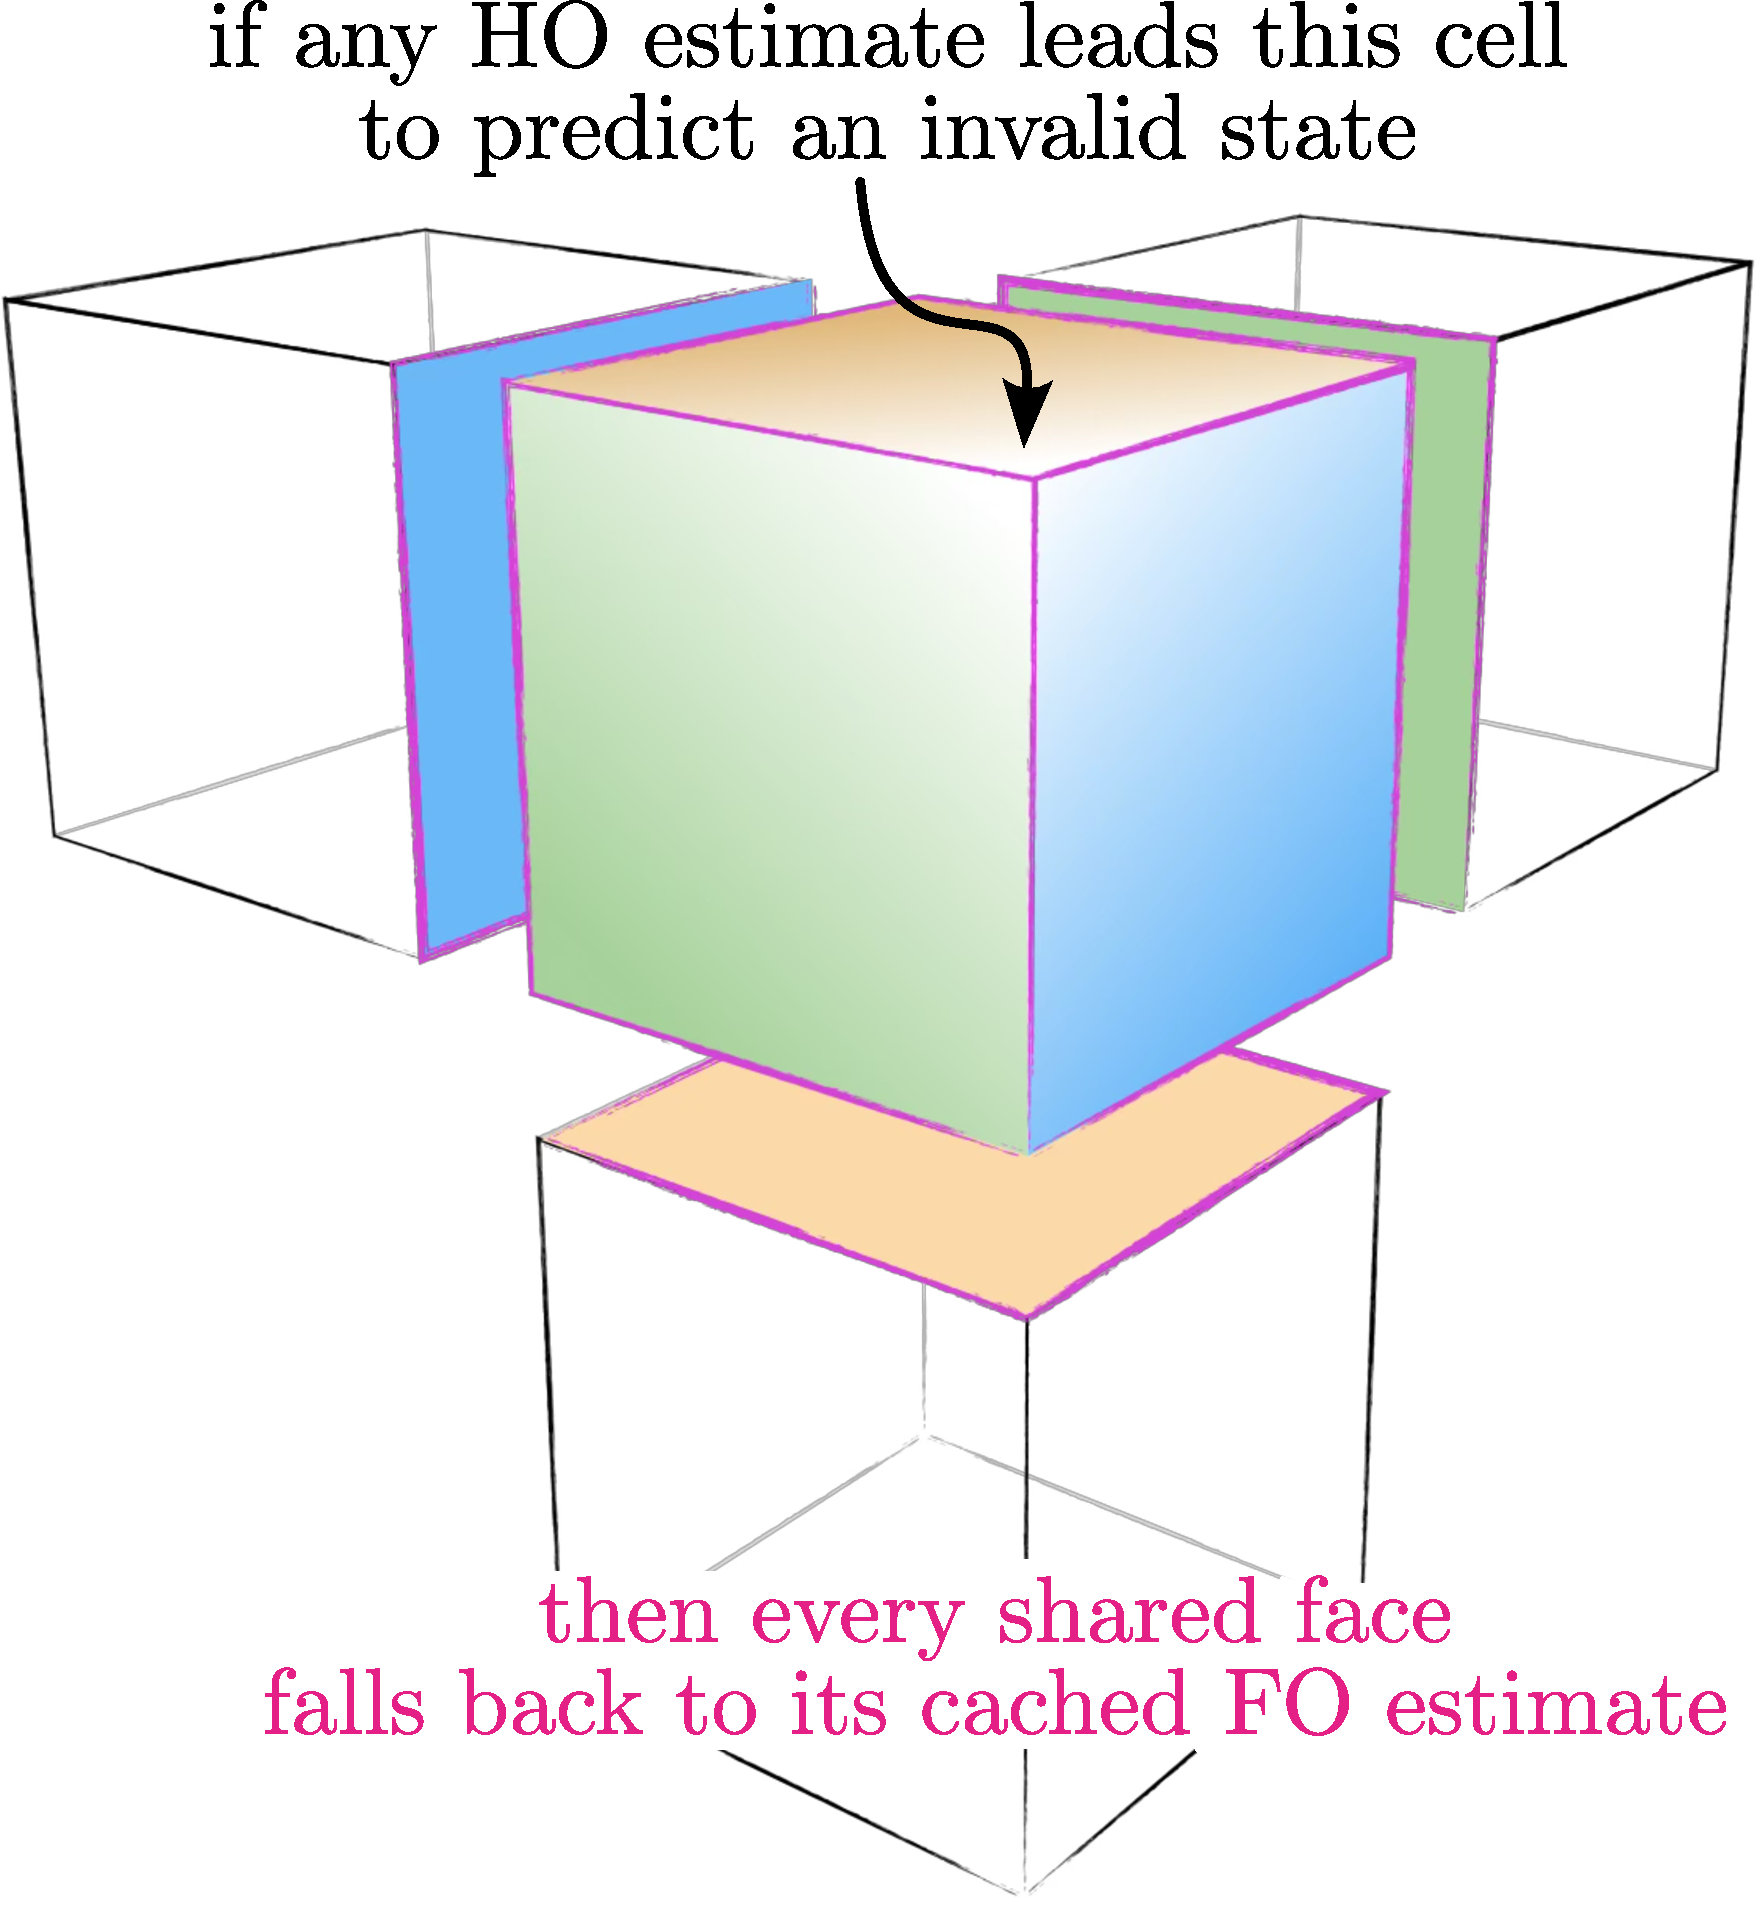
\includegraphics[width=0.55\linewidth]{figures/quokka-mhd/schematics/fofc.pdf}
    \caption{Illustration of the first-order flux correction (FOFC) scheme. If the predicted cell-centred state of a cell computed using a high-order method (HO) is flagged as invalid after either the first or second RK stage, the fluxes on each of its faces and the EMFs on each of its edges are replaced by first-order (FO) estimates, and the update is recomputed both the flagged cell, for all of its neighbours that share a face or edge whose flux or EMF has been replaced.}
    \label{fig:fofc}
\end{figure}

This completes the update cycle. Note that if no flux replacements take place in either of the RK stages, then this update reduces to a standard RK2-SSP method. Conversely, if we replace the HO fluxes with FO fluxes during both RK stages, this update procedure reduces to a simple first order in time forwards Euler update, with the fluxes and EMFs in turn determined from a first order in space interpolation procedure. Thus the entire scheme consistently falls back to first order if it encounters a bad state, hence our description of the scheme as FOFC. However, our procedure can also yield an intermediate approximation if the HO flux is replaced by a FO flux at one but not both of the RK stages. In this case we obtain an estimate that is intermediate in terms of accuracy.

% Borris correction: MHD eqns make the assumption that 

\subsection{AMR considerations}
\label{sec:methods:amr}

The scheme we have just described is naturally extensible to AMR. \textsc{Quokka} uses \citet{Berger84a} block-structured AMR with \citet{Berger89a} adaptive time stepping as implemented in the \textsc{AMReX} library \citep{Zhang19b}, and applying this approach to our MHD scheme requires two additional ingredients: a method to refine or coarsen the face-centred magnetic field quantities when increasing or decreasing the resolution, and a method to correct for mismatches in the flux across coarse-fine level boundaries. For refinement and coarsening, \textsc{Quokka} uses the divergence-preserving interpolator introduced by \citet{Vanella10a}, and implemented as part of \textsc{AMReX}. This guarantees that the discrete magnetic divergence remains zero when we add or remove levels, or when we fill ghost zones. For flux mismatches, we implement the flux-correction scheme described by \citet{Balsara01a}, and also used in the \textsc{orion2} code \citep{Li12a}. Briefly, this scheme corrects the magnetic field estimate on coarse cell faces that lie at coarse-fine boundaries to ensure that they are updated using the same EMFs as were used to update the fine cell faces, thereby maintaining zero divergence across coarse-fine interfaces.

\section{Comparison of Schemes}
\label{sec:performance}

\autoref{sec:methods:emf} introduces three schemes for extrapolating EMFs to cell edges and two for averaging them together, each of which can be combined with PC, PLM, PPM, and PPM-EP interpolation. Our next goal is to compare the performance of these schemes. To this end, we first test their convergence in simulating linear MHD waves in \autoref{sec:performance:waves} and their ability to capture magnetised shocks in \autoref{sec:performance:brio-wu}, followed by \autoref{sec:performance:orszag-tang} where we test their stability and accuracy in a challenging multidimensional, non-linear problem. We then evaluate their relative speed in \autoref{sec:performance:speed}, before making final recommendations in \autoref{sec:performance:summary}. Unless noted otherwise, all the tests reported in this section and the next one were carried out on the Setonix machine at the Pawsey Supercomputing Centre in Western Australia. Each node of this machine provides four AMD Instinct MI-250X GPU cards with two logical GPUs per card; nodes are linked with HPE Slingshot interconnects.

\subsection{Convergence for linear waves}
\label{sec:performance:waves}

We first test the basic accuracy and convergence of our schemes for two simple linear waves: a linearly-polarised Alfv\'en wave and a fast wave. For both waves, we consider a uniform background state 
\begin{align}
    \mVector{S}_\mathrm{c}^{\{0\}}
        = \begin{Bmatrix}
                \rho \\
                \rho \mVector{u} \\
                e_\mathrm{tot} \\
                \mVector{b}
            \end{Bmatrix}
        = \begin{Bmatrix}
                \rho_0 \\
                \mVector{0} \\
                p_0 / (\gamma-1) + b_0^2/2 \\
                b_0 \mVectorUnit{n}_{0}
            \end{Bmatrix}
\end{align}
where $\rho_0$, $p_0$, $b_0$, and $\mVectorUnit{n}_{0}$ are the background density, pressure, magnetic field magnitude, and magnetic field direction, and $\gamma$ is the adiabatic index. We consider a perturbation with wave vector $\mVector{k}$ in a cubical periodic domain of size $L$ on side; we define $\mVectorUnit{n}_k = \mVector{k}/k$ as the unit vector in the direction of $\mVector{k}$, and $\tilde{\mVector{k}} = \mVector{k}L/2\pi$ as the box-normalised wave vector. Continuity requires that all elements of $\tilde{\mVector{k}}$ be integer-valued.

For the Alfv\'en wave, we then consider a perturbation to the background state
\begin{align}
    \delta \mVector{S}_\mathrm{c}^{\{A\}}
        = \delta_{a} \cos\sbrac{\omega t - \mVector{k}\cdot\mVector{x}}
        \begin{Bmatrix}
            0 \\
            -c_\mathrm{A} \mVectorUnit{n}_\perp \\
            \delta_{a} c_\mathrm{A}^2 \\
            b_0 \mVectorUnit{n}_\perp
        \end{Bmatrix}
    ,
\end{align}
where $\delta_{a}$ is a small dimensionless number giving the amplitude of the perturbation, $c_\mathrm{A} = b_0 / \sqrt{\rho_0}$ is the Alfv\'en speed, $\mVectorUnit{n}_\perp$ as a unit vector in the direction $\pm (\mVectorUnit{n}_{0} \times \mVectorUnit{n}_{k})$ (or just orthogonal to $\mVectorUnit{n}_{k}$ in the singular case where $\mVectorUnit{n}_{0} \parallel \mVectorUnit{n}_{k}$), $\omega = c_\mathrm{A} k \cos\theta$ is the angular frequency, and $\theta = \cos^{-1}[\mVectorUnit{n}_{0} \cdot \mVectorUnit{n}_{k}]$ is the angle between the background magnetic field and wave vector. Similarly, for the fast wave, we consider a perturbation
\begin{align}
    \delta\mVector{S}_\mathrm{c}^{\{\mathrm{fm}\}}
        &= \delta_{a} \cos\sbrac{\omega t - \mVector{k}\cdot\mVector{x}}
        \nonumber \\
        &\nquad[2] \begin{Bmatrix}
            \phi_1 \rho_0 \\
            c_\mathrm{fm} (
                    \phi_1 \mVectorUnit{n}_{k} - \phi_2 \mVectorUnit{n}_\perp
                ) \\
            \phi_1 p_0 \gamma / (\gamma-1)
                + b_0^2\sin\theta
                + \delta_{a} \rbrac{
                    b_0^2/2
                    + \rho_0 c_\mathrm{fm}^2 \rbrac{\phi_1^2 + \phi_2^2}
                } \\
            b_0 \mVectorUnit{n}_\perp
        \end{Bmatrix}
    ,
\end{align}
where $\mVectorUnit{n}_\perp$ is a unit vector orthogonal to $\mVectorUnit{n}_{k}$ and lying in the plane formed by $\mVectorUnit{n}_{k}$ and $\mVectorUnit{n}_{0}$,
\begin{align}
    c_\mathrm{fm}^2
        = \frac{1}{2} \rbrac{
            c_\mathrm{s}^2 + c_\mathrm{A}^2 + \rbrac{
                \rbrac{c_\mathrm{s}^2 + c_\mathrm{A}^2}^2 - 4 c_\mathrm{s}^2 c_\mathrm{A}^2 \cos^2\theta
            }^{1/2}
        }
\end{align}
is the fast magnetosonic speed, $c_\mathrm{s} = \sqrt{\gamma p_0/\rho_0}$ is the sound speed, $\omega = c_\mathrm{fm} k$ is the angular frequency, and the geometry factors $\phi_1$ and $\phi_2$ are given by
\begin{align}
    \phi_1
        &= \frac{c_\mathrm{fm}^2 - c_\mathrm{A}^2 \cos^2\theta}{c_\mathrm{fm}^2 \sin\theta} \\
    \phi_2
        &= \rbrac{\frac{c_\mathrm{A}}{c_\mathrm{fm}}}^2 \cos\theta
    .
\end{align}

For the tests comparing scheme convergence rates that we carry out in this section, we consider grid-aligned waves described by $\tilde{\mVector{k}} = \{1,0,0\}$; for the Alfv\'en wave test we use $\tilde{\mVector{n}}_0 = \{1,0,0\}$ and  $\tilde{\mVector{n}}_\perp = \{0,0,1\}$ (corresponding to $\theta = 0$), while for the fast wave test we use $\tilde{\mVector{n}}_0 = \{0,1,0\}$ and $\tilde{\mVector{n}}_\perp = \{0,1,0\}$ (so that $\theta = 90^\circ$). This orientation allows us to use a grid that expands only in a single direction, which is convenient for convergence testing where we wish to go to very high resolution for a large number of code options; we present results showing the accuracy of our code for non-grid-aligned waves in \autoref{sec:tests}. For all tests we adopt $\rho_0 = b_0 = 1$, $p_0 = 1/\gamma$ (corresponding to $c_\mathrm{s} = 1$), $\gamma = 5/3$, and $\delta_{a} = 10^{-6}$. We initialise the simulation\footnote{
    Initialising the magnetic field requires some care to ensure \mbox{$\nabla\cdot\mVector{b} = 0$} to machine precision under our chosen stencil. To initialise the magnetic field we analytically compute the vector potential corresponding to the magnetic field at centres of cell edges -- the same locations at which we store the EMFs. We then compute curl of the vector potential using a centred stencil to generate the magnetic field at the face of each cell.
} to state $\mVector{S}_\mathrm{c}^{\{0\}} + \delta\mVector{S}_\mathrm{c}^{A}$ (for the Alfv\'en wave test) or $\mVector{S}_\mathrm{c}^{\{0\}} + \delta\mVector{S}_\mathrm{c}^{\{\mathrm{fm}\}}$ (for the fast wave test) evaluated at $t=0$ and simulate to time $t = 2\pi/\omega$, corresponding to a single wave period, so that the final and initial states should be identical. We run simulations of both waves in a domain of size $L=1$ using uniform grids of size $\{N, 8, 8\}$, with $N$ varying from 16 to 2048 in factor of 2 steps, using all possible combinations of EMF reconstruction scheme (\autoref{sec:methods:emf:reconstruction}), EMF averaging scheme (\autoref{sec:methods:emf:averaging}), and interpolation scheme (PLM, PPM, and PPM-EP); we list the full set of tested scheme combinations in \autoref{tab:linear_convergence}.

For each simulation we measure the relative $L_1$ error. We define this by first defining the absolute $L_1$ error for each quantity $q$ in the state vector $\mVector{S}_\mathrm{c}$ as
\begin{align}
    \mbox{error}_q
        = \frac{1}{N_q} \sum_{\forall i, j, k} \bigg|
            q_\mathrm{exact}\EvalAtH{i}{j}{k}
            - q_\mathrm{sim}\EvalAtH{i}{j}{k}
        \bigg|
    ,
\end{align}
where $q_\mathrm{sim}\EvalAtH{i}{j}{k}$ and $q_\mathrm{exact}\EvalAtH{i}{j}{k}$ are the simulation-predicted and exact values at coordinate $(i, j, k)$ (the indexing is determined by whether $q$ is stored at cell-centres or face-centres), $N_q$ is the number of cell centres or faces for that quantity, and the sums run over all centres or faces. We similarly define the normalisation for that quantity as
\begin{align}
    \mbox{norm}_q
        = \frac{1}{N_q} \sum_{\forall i, j, k} \bigg|
            q_\mathrm{exact}\EvalAtH{i}{j}{k}
        \bigg|
    ,
\end{align}
and then define the relative $L_1$ error as
\begin{align}
    \epsilon
        = \rbrac{\frac{
                    \sum_{\forall q} \mbox{error}_q^2 N_q^2
                }{
                    \sum_{\forall q} \mbox{norm}_q^2 N_q^2
            }}^{1/2}
    . \label{defn:error}
\end{align}
We plot this error as a function of resolution for all schemes in \autoref{fig:linear_wave_convergence}.

\begin{figure}
    \centering
    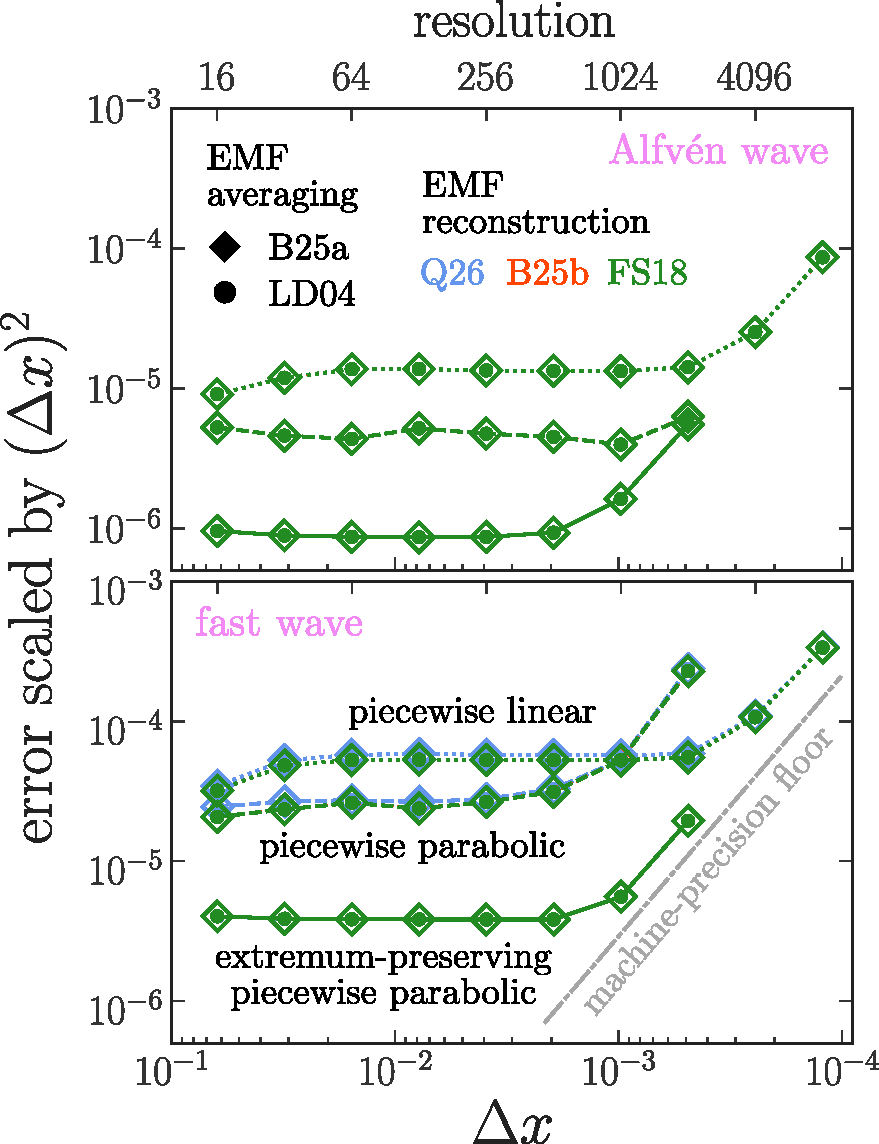
\includegraphics[width=0.65\linewidth]{figures/quokka-mhd/results/wave_convergence.pdf}
    \caption{Convergence tests for Alfv\'en waves (top) and fast waves (bottom). In both panels, lines show the $L^1$ error (\autoref{defn:error}) compensated by grid spacing $(\Delta x)^2$, as a function of grid spacing; thus second-order convergence corresponds to a flat line in these plots. Blue, red, and green colours show the Q26, \citetalias{Balsara25a}, and \citetalias{Felker18a} EMF reconstruction schemes, respectively; diamond and circle markers indicate \citetalias{Londrillo04a} and \citetalias{Balsara25b} EMF averaging, respectively; dotted, dashed, and solid lines show PLM, PPM, and PPM-EP reconstruction, respectively. Because the results are nearly the same for all EMF averaging and reconstruction schemes, in many cases points are not visible because they are directly under other points. The dashed grey line labelled ``machine precision floor'' indicates where the error deviates from $\mathcal{O}((\Delta x)^{-2})$ scaling because the difference between the numerical and analytic solution is comparable to the numerical precision imposed by machine arithmetic.}
    \label{fig:linear_wave_convergence}
\end{figure}

\begin{table}
\centering
\caption{Best-fit parameters for error versus resolution (\autoref{eq:err_vs_resolution}) for different combinations of EMF reconstruction scheme, EMF averaging scheme, interpolation type, and wave type.
\label{tab:linear_convergence}}
\begin{tabular}{llrrr}
\hline\hline
Reconstruction & Averaging & $\log \alpha_0$ & $\alpha_1$ & $\log \alpha_2$ \\
\hline
\multicolumn{5}{c}{Alfv\'en waves, PLM interpolation} \\
\hline
B25 & B25 & $-5.231$ & 1.840 & $-11.984$ \\
B25 & LD04 & $-5.231$ & 1.840 & $-11.983$ \\
FS17 & B25 & $-5.231$ & 1.840 & $-11.983$ \\
FS17 & LD04 & $-5.231$ & 1.840 & $-11.983$ \\
Q26 & B25 & $-5.231$ & 1.840 & $-11.983$ \\
Q26 & LD04 & $-5.231$ & 1.840 & $-11.983$ \\
\hline
\multicolumn{5}{c}{Fast waves, PLM interpolation} \\
\hline
B25b & B25a & $-4.742$ & 1.791 & $-11.528$ \\
B25b & LD04 & $-4.742$ & 1.791 & $-11.528$ \\
FS17 & B25a & $-4.742$ & 1.791 & $-11.528$ \\
FS17 & LD04 & $-4.742$ & 1.791 & $-11.528$ \\
Q26 & B25a & $-4.707$ & 1.790 & $-11.640$ \\
Q26 & LD04 & $-4.707$ & 1.790 & $-11.640$ \\
\hline
\multicolumn{5}{c}{Alfv\'en waves, PPM interpolation} \\
\hline
B25b & B25a & $-5.197$ & 2.070 & $-11.903$ \\
B25b & LD04 & $-5.197$ & 2.070 & $-11.903$ \\
FS18 & B25a & $-5.197$ & 2.070 & $-11.903$ \\
FS18 & LD04 & $-5.197$ & 2.070 & $-11.903$ \\
Q26 & B25a & $-5.197$ & 2.070 & $-11.903$ \\
Q26 & LD04 & $-5.197$ & 2.070 & $-11.903$ \\
\hline
\multicolumn{5}{c}{Fast waves, PPM interpolation} \\
\hline
B25b & B25a & $-4.759$ & 1.936 & $-10.303$ \\
B25b & LD04 & $-4.758$ & 1.937 & $-10.303$ \\
FS18 & B25a & $-4.760$ & 1.936 & $-10.303$ \\
FS18 & LD04 & $-4.760$ & 1.936 & $-10.303$ \\
Q26 & B25a & $-4.614$ & 1.997 & $-10.298$ \\
Q26 & LD04 & $-4.613$ & 1.998 & $-10.298$ \\
\hline
\multicolumn{5}{c}{Alfv\'en waves, PPM-EP interpolation} \\
\hline
B25b & B25a & $-5.962$ & 2.049 & $-11.883$ \\
B25b & LD04 & $-5.962$ & 2.049 & $-11.883$ \\
FS17 & B25a & $-5.962$ & 2.049 & $-11.883$ \\
FS17 & LD04 & $-5.962$ & 2.049 & $-11.883$ \\
Q26 & B25a & $-5.962$ & 2.049 & $-11.883$ \\
Q26 & LD04 & $-5.962$ & 2.049 & $-11.883$ \\
\hline
\multicolumn{5}{c}{Fast waves, PPM-EP interpolation} \\
\hline
B25b & B25a & $-5.351$ & 2.035 & $-11.343$ \\
B25b & LD04 & $-5.351$ & 2.035 & $-11.343$ \\
FS17 & B25a & $-5.351$ & 2.035 & $-11.343$ \\
FS17 & LD04 & $-5.351$ & 2.035 & $-11.343$ \\
Q26 & B25a & $-5.352$ & 2.035 & $-11.343$ \\
Q26 & LD04 & $-5.352$ & 2.035 & $-11.343$ \\
\hline\hline
\end{tabular}
\end{table}

As the plot shows, and as expected, we find that the error decreases as a powerlaw in the $N$, for small $N$, before reaching a minimum error imposed by the finite precision of machine arithmetic and / or the fact that the analytic solution is only accurate to first order in the perturbation amplitude $\delta_{a}$. We therefore carry out a simple $\chi^2$ fit for the $L^1$ errors we measure at different resolutions of each scheme, using a functional form
\begin{align}
    \epsilon(N)
        = \rbrac{\rbrac{\alpha_0 N^{-\alpha_1}}^2 + \alpha_2^2}^{1/2}
    , \label{eq:err_vs_resolution}
\end{align}
where the error normalisation $\alpha_0$, floor value $\alpha_2$, and convergence rate $\alpha_1$ are parameter to be fit. We report the best-fit values for all combinations of scheme in \autoref{tab:linear_convergence}.

As the figure and tabulated data show, the error normalisations, floor values, and convergence rates are nearly identical for all combinations of EMF reconstruction and averaging scheme. These quantities depend only on the reconstruction type (PLM, PPM, or PPM-EP), and all schemes achieving roughly second-order convergence, $\alpha_1 \approx 2$ -- which is expected behaviour given that we have not implemented the extra interpolation steps that would be required to reach higher-order \citep[e.g.,][]{Felker18a, Balsara25a}. The order of interpolation mostly appear to affect the normalisation of the error scaling. We therefore conclude that all of the reconstruction and averaging schemes perform nearly-identically for linear waves, and that the differences in interpolation scheme behave as expected for each of them.

\subsection{Magnetised shocks: the Brio-Wu shock tube}
\label{sec:performance:brio-wu}

Our second comparison between the schemes is the classic \citet{Brio88a} shock tube test. In this test we start with a discontinuity at $x=0$, with the states at $x<0$ and $x>0$ defined by, respectively,
\begin{align}
    \begin{Bmatrix}
        \rho \\
        u_1 \\
        u_2 \\
        u_3 \\
        e_\mathrm{tot} \\
        b_1 \\
        b_2 \\
        b_3
    \end{Bmatrix}_L
        = \begin{Bmatrix}
            1 \\
            0 \\
            0 \\
            0 \\
            1.78125\\
            0.75 \\
            1 \\
            0
        \end{Bmatrix}
    \, \, \mbox{and}\, \, 
    \begin{Bmatrix}
        \rho \\
        u_1 \\
        u_2 \\
        u_3 \\
        e_\mathrm{tot} \\
        b_1 \\
        b_2 \\
        b_3
    \end{Bmatrix}_R
        = \begin{Bmatrix}
            0.125 \\
            0 \\
            0 \\
            0 \\
            0.88125\\
            0.75 \\
            -1\\
            0
        \end{Bmatrix}        
\end{align}
The gas is adiabatic with index $\gamma=2$. We run this problem at a resolution of $512 \times 8 \times 8$ to time $t = 0.1$ over a domain $x_1 \in [0, 1]$ using all six possible combinations of EMF reconstruction and averaging scheme (\citetalias{Felker18a}, \citetalias{Balsara25a}, and Q26, together with \citetalias{Londrillo04a} and \citetalias{Balsara25b}). We use PPM-EP interpolation for all of these tests.

We show the results in \autoref{fig:bw-profiles}, comparing to a reference solution from \citetalias{Felker18a}. We find that all schemes reproduce the reference solution extremely well, properly capturing all of the features. The choice of EMF averaging scheme makes no noticeable difference. The EMF reconstruction scheme matters slightly more, with the Q26 scheme showing somewhat more ringing in the region between the intermediate compound wave and the contact discontinuity (see inset in \autoref{fig:bw-profiles}). However, the differences are small.

\begin{figure}
    \centering
    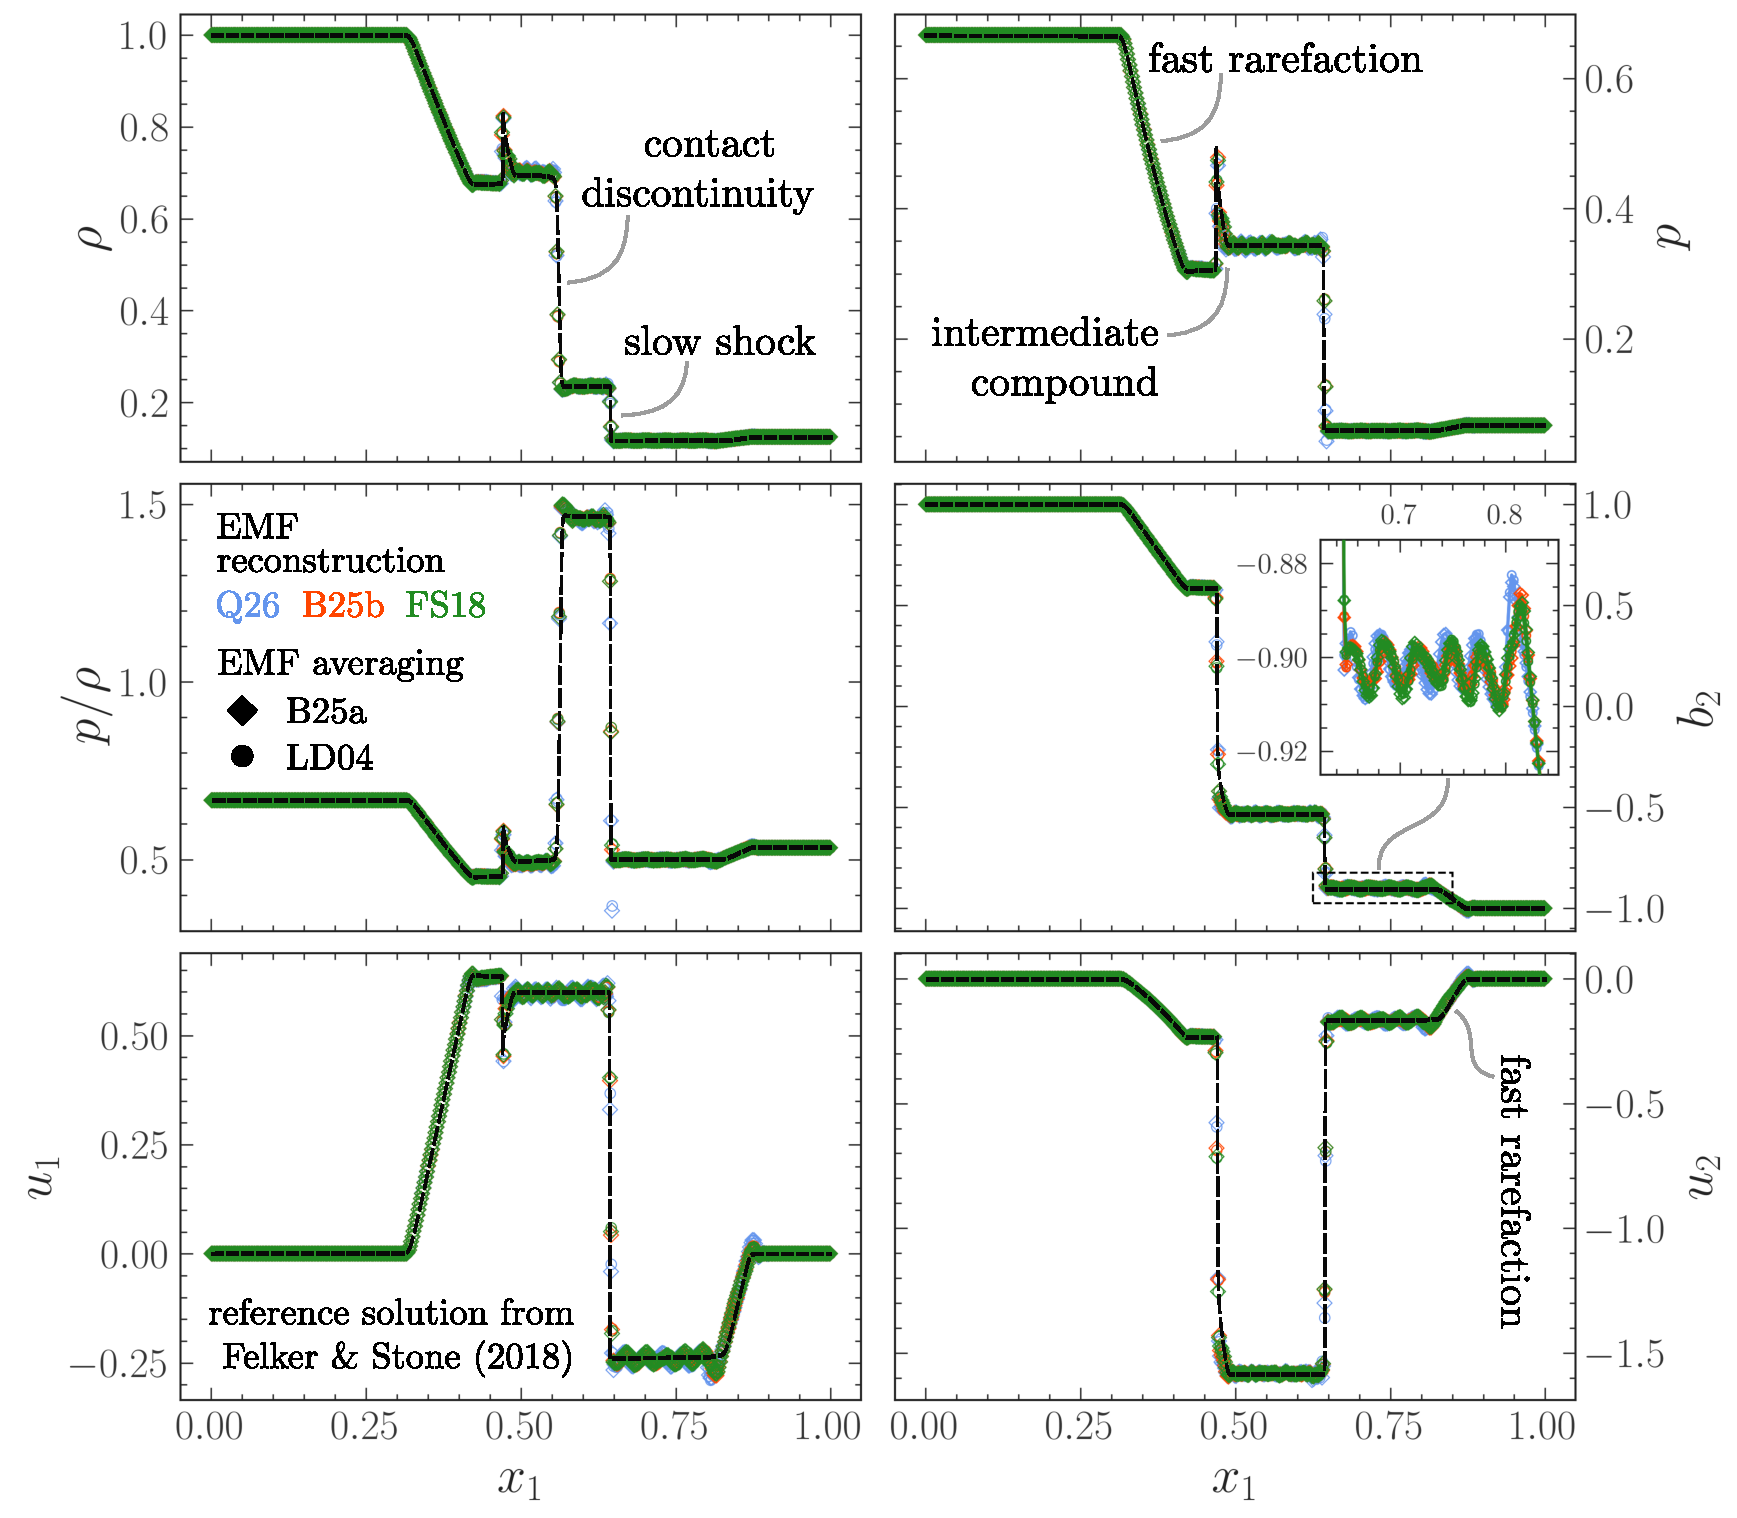
\includegraphics[width=\linewidth]{figures/quokka-mhd/results/bw-profiles.pdf}
    \caption{Results for the \citet{Brio88a} shock tube test. The panels show, from top left and proceeding across and down, density, pressure, ratio of pressure to density, magnetic field in the $x_2$ direction, and velocity in the $x_1$ and $x_2$ directions. Solutions generated using Q26, \citetalias{Balsara25a}, and \citetalias{Felker18a} EMF reconstruction are shown in blue, red, and green, respectively, while those using \citetalias{Balsara25b} and \citetalias{Londrillo04a} EMF averaging are shown by diamond and circular symbols, respectively. The dashed black line show the reference solution, which we take from \citetalias{Felker18a}. Annotations indicate the different discontinuities in the solution.}
    \label{fig:bw-profiles}
\end{figure}

\subsection{Stability and accuracy for non-linear problems}
\label{sec:performance:orszag-tang}

To test the stability of our scheme combinations, we use the Orszag-Tang test \citep{OrszagTang1979}. This is a two-dimensional non-linear MHD vortex that evolves into interacting shocks and current sheets and tests the Riemann solver and the EMF reconstruction schemes. We run all tests at a high resolution of $1024\times 1024 \times 8$ and to time $t=1$, long enough for the system to mix and develop interacting shock waves, in order to test the robustness of the schemes in a high-stress problem. All our tests for this section use eight GPUs.

\begin{figure}
    \centering
    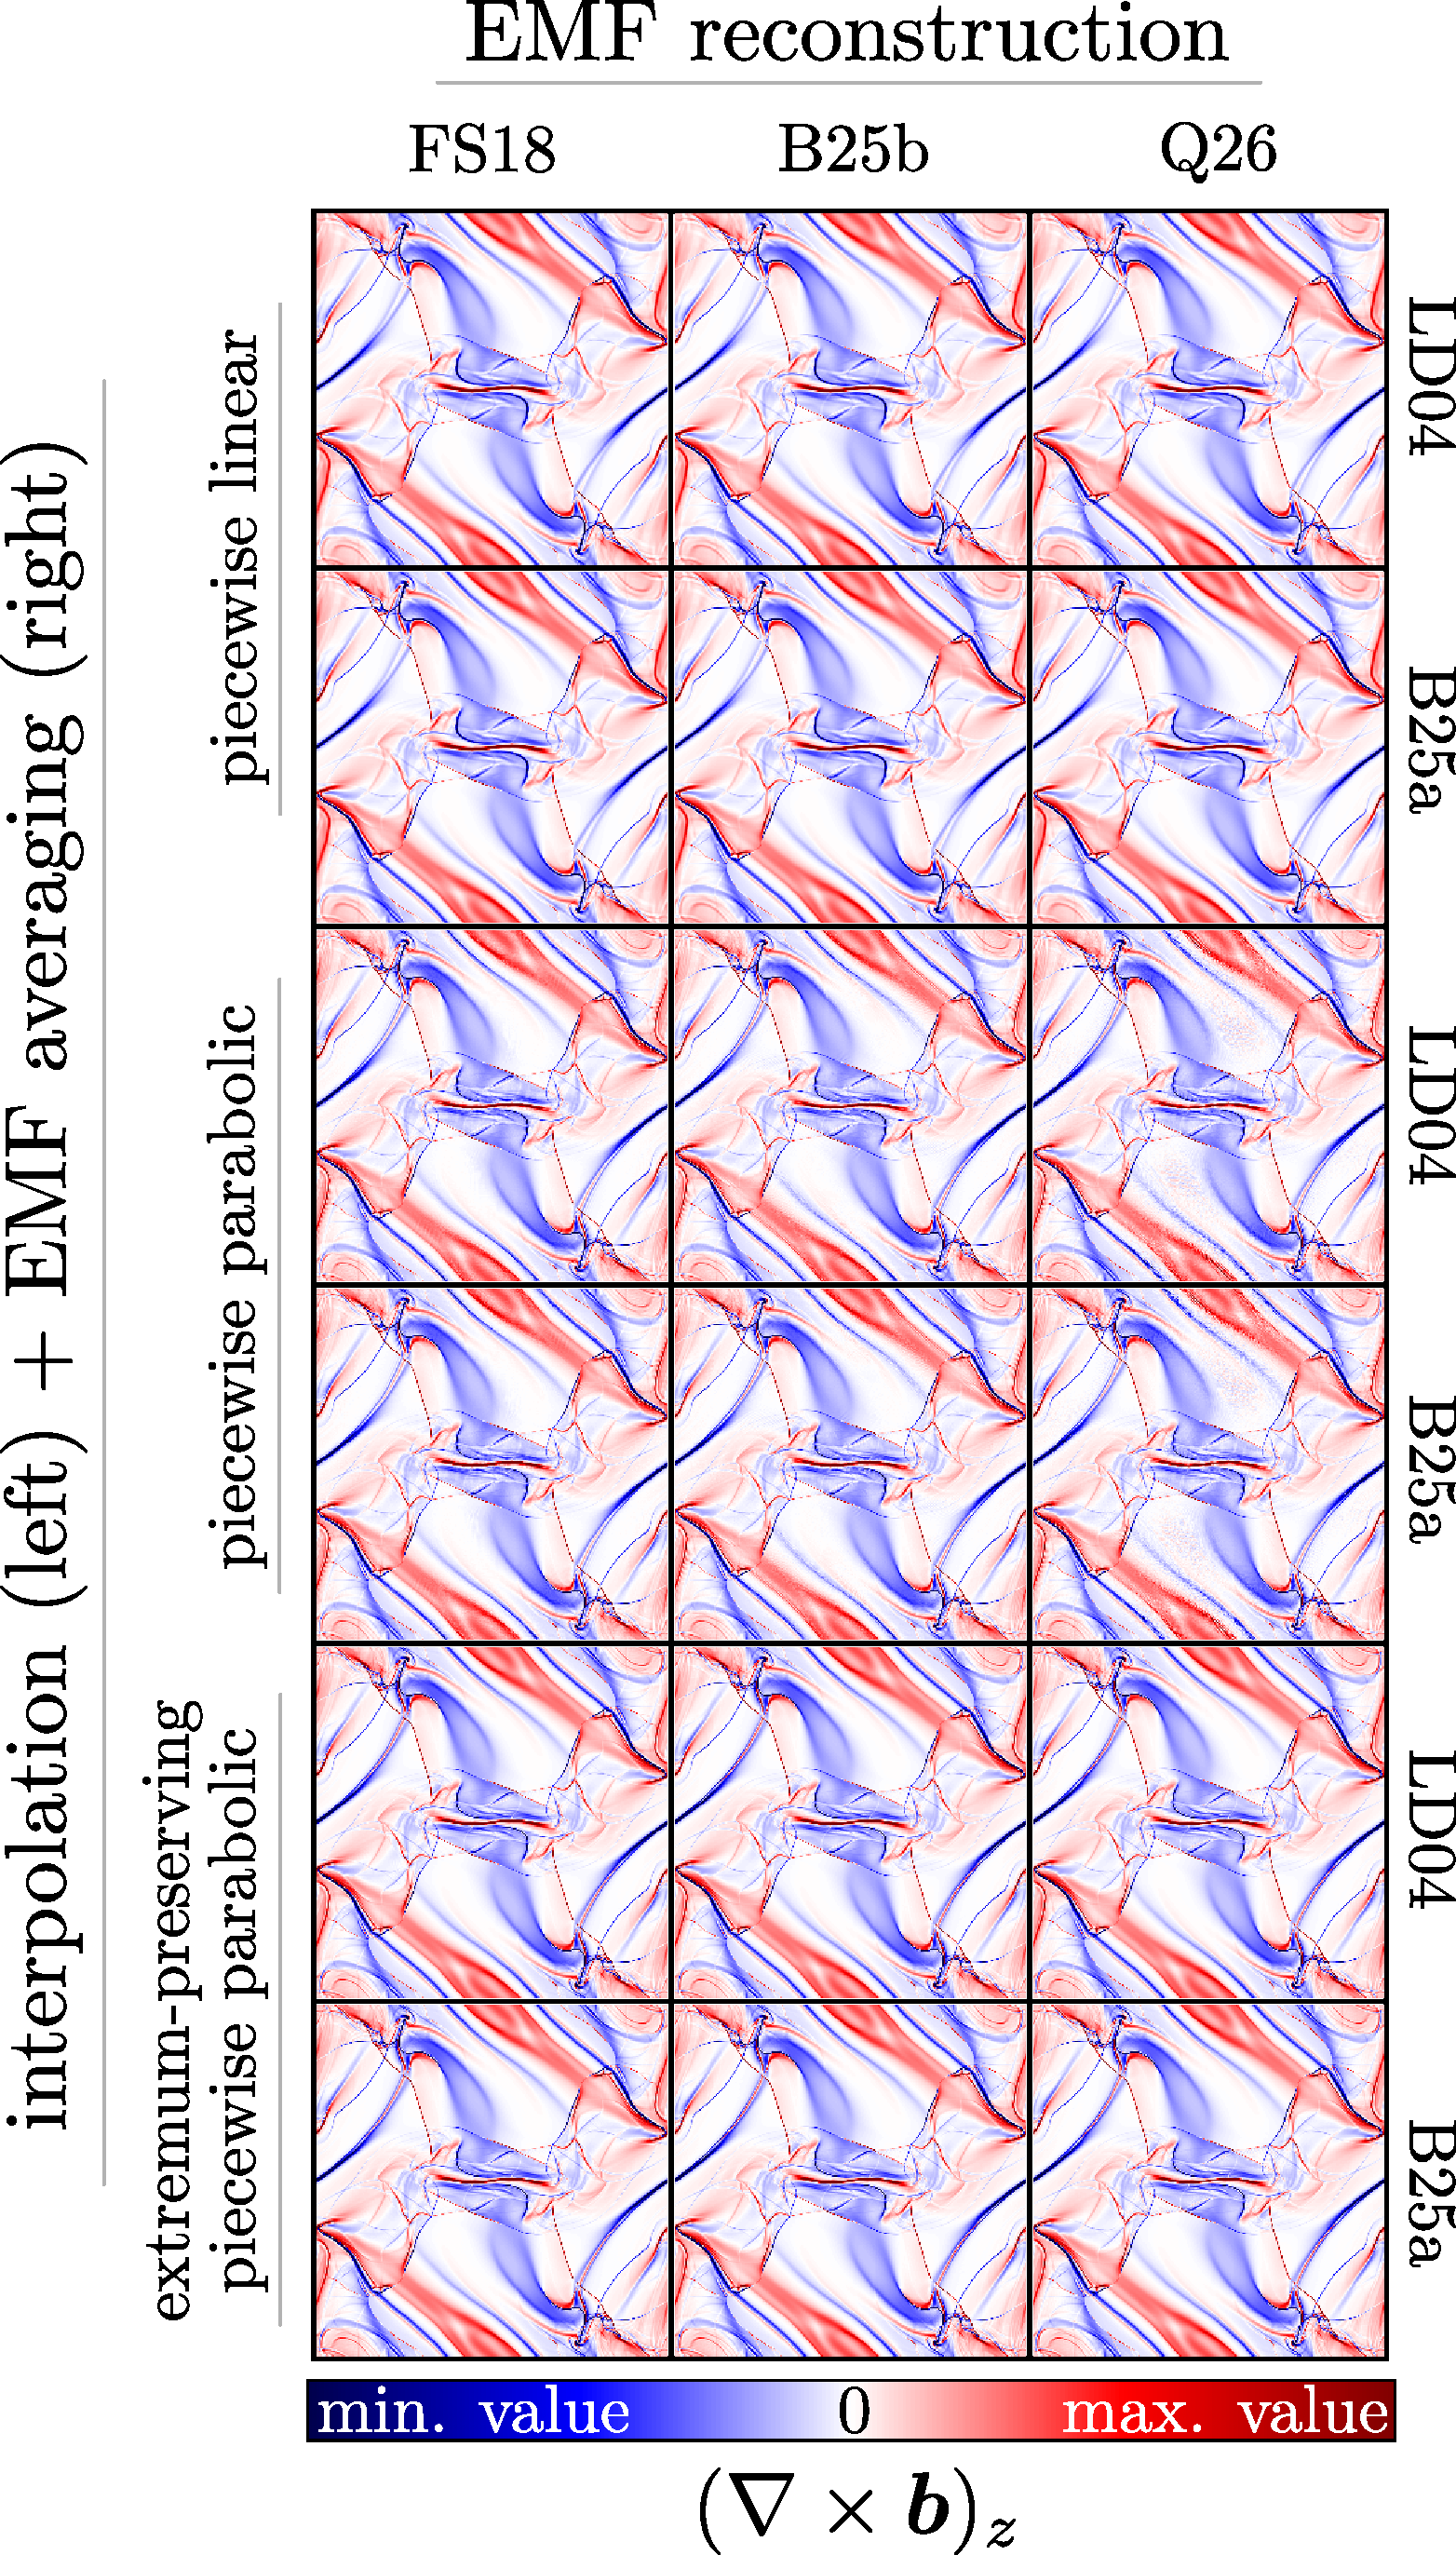
\includegraphics[width=0.75\linewidth]{figures/quokka-mhd/results/ot-schemes-lores.pdf}
    \caption{Slice plots taken through the midplane of the Orszag-Tang problem for each of combination of interpolation (labelled on the left), EMF reconstruction (labelled on the top), and EMF averaging (labelled on the right). The size of the computational domain shown is $1\times 1$ in dimensionless units, and we plot the out-of-plane component of the current density at $t = 0.5$.}
    \label{fig:OT_current}
\end{figure}

We show the current density in the out-of-plane direction at $t=0.5$ that we obtain for this problem in \autoref{fig:OT_current}, for each combination of EMF reconstruction scheme, EMF averaging scheme, and interpolation type that we tested. From this figure we can make a few observations. First, the most obvious differences are between interpolation methods -- PLM (top two rows) versus PPM (middle two rows) versus PPM-EP (bottom two rows). The PLM results are noticeably smoother and less noisy, while the PPM and PPM-EP results both have some clear ringing, though more for PPM than PPM-EP. Second, the differences between EMF averaging method (\citetalias{Londrillo04a} versus \citetalias{Balsara25b}) are minimal -- the first and second rows are nearly identical, as are the third and fourth, and fifth and sixth. Finally, the choice of EMF reconstruction method (\citetalias{Felker18a} versus \citetalias{Balsara25a} versus Q26) makes almost no difference with PLM interpolation (top two rows), and does not change the large scale characteristics of the solution with PPM or PPM-EP, but does make a difference to the pattern of ringing with these higher-order methods. For example, with PPM interpolation (middle two rows), the \citetalias{Felker18a} method (left column) shows less ringing than \citetalias{Balsara25a}, which in turn shows less ringing than Q26, and in going between \citetalias{Balsara25a} and Q26 (middle and right columns) the orientation of the ringing pattern rotates by $\approx 90^\circ$.

\begin{table}
\centering
\caption{Number of time steps required to reach $t=1$ (third column) and number of first-order flux corrections (right column) for the Orszag-Tang test using different schemes for interpolation, EMF reconstruction (first column), and averaging (second column).
\label{tab:ot_steps}
}
\begin{tabular}{llcr}
\hline\hline
Reconstruction & Averaging & N. time steps & N. FOFC steps  \\
\hline
\multicolumn{4}{c}{PLM interpolation} \\
\hline
FS18 & LD04  &  15985 & 0 \\
FS18 & B25a  &  15989 & 0 \\
B25b & LD04  &  16005 & 0 \\
B25b & B25a  &  15948 & 0 \\
Q26  & LD04  & 18335 & 0 \\
Q26  & B25a  &  19339 & 0 \\
\hline
\multicolumn{4}{c}{PPM interpolation} \\
\hline
FS18 & LD04  &  16149 & 0 \\
FS18 & B25a  &  16153 & 0 \\
B25b & LD04  &  16210 & 0 \\
B25b & B25a  &  16282 & 0 \\
Q26  & LD04  &   41231 & 0 \\
Q26  & B25a  &  \,$^{\dagger}$ & 0 \\
\hline
\multicolumn{4}{c}{PPM-EP interpolation} \\
\hline
FS18 & LD04  &  16295 & 0 \\
FS18 & B25a  &  16286 & 0 \\
B25b & LD04  &  16483 & 0 \\
B25b & B25a  &  16527 & 0 \\
Q26  & LD04  & \,$^{\ddagger}$ & 80 \\
Q26  & B25a  & \,$^{\ddagger}$ & 80 \\
\hline\hline
\end{tabular}
\vspace{0.5ex}
\begin{flushleft}
\footnotesize
$^{\dagger}$~Run terminated early because the time step became prohibitively small.\\
$^{\ddagger}$~Run became numerically unstable and crashed before reaching the final time.
\end{flushleft}
\end{table}

These differences in the amount of ringing manifest at later times as differences in stability. While all schemes run successfully up to the time shown in \autoref{fig:OT_current}, not all of them are able to continue up to $t=1$, or require the same number of time steps to reach this point. We report in \autoref{tab:ot_steps} the number of time steps that each scheme required to reach $t=1$ and the number of first-order flux corrections that occurred; single and double daggers indicate that a given scheme terminated before reaching $t=1$ because the time step became prohibitively small or because the scheme crashed, respectively. We see that the Q26 scheme behaves comparably to the others for PLM, albeit requiring slightly more time steps, but that it either requires many more time steps or fails altogether for the higher-order interpolation methods. By contrast, the results for the \citetalias{Felker18a} and \citetalias{Balsara25a} reconstruction schemes, and for both \citetalias{Londrillo04a} and \citetalias{Balsara25b} averaging, are nearly identical. Thus the Q26 scheme provides comparable quality results to the others, but appears slightly less table at high order.

\subsection{Performance and scaling}
\label{sec:performance:speed}

\begin{table}
\centering
\caption{Weak scaling test results for different schemes and GPU counts in a test with $128^3$ cells per GPU. The first two columns indicate the EMF reconstruction and averaging schemes, and the remaining columns show results as a function of GPU count. Entries in the remaining columns report the cell advance time $t_\mathrm{adv}$ in units of ns, defined as the amount of GPU time required to advance a single cell through one time step, and different GPU counts $N_\mathrm{GPU}$.}
\label{tab:weak_scaling_zone_update_times_ngpu}
\begin{tabular}{llrrrr}
\hline\hline
& & \multicolumn{4}{c}{$t_\mathrm{adv}/\mathrm{ns}$ at $N_\mathrm{GPU}=\cdots$} \\
Reconstruction & Averaging & 1 & 8 & 64 & 512 \\
\hline
FS18 & LD04  & 34.65 & 34.94 & 36.84 & 48.51 \\
FS18 & B25a  & 34.76 & 34.88 & 36.74 & 39.83 \\
B25b & LD04  & 27.58 & 28.71 & 31.44 & 37.69 \\
B25b & B25a  & 27.65 & 28.94 & 31.58 & 46.07 \\
Q26  & LD04  & 21.19 & 23.12 & 27.24 & 30.58 \\
Q26  & B25a  & 21.23 & 23.02 & 27.01 & 29.44 \\
\hline\hline
\end{tabular}
\end{table}
\begin{table*}
\centering
\caption{Same as \autoref{tab:weak_scaling_zone_update_times_ngpu}, but now showing the advance times measured for strong scaling in a test with a fixed $512^3$ cells.}
\label{tab:strong_scaling_zone_update_times_ngpu}
\begin{tabular}{llrrrrrrrr}
\hline\hline
& & \multicolumn{8}{c}{$t_\mathrm{adv}/\mathrm{ns}$ at $N_\mathrm{GPU}=\cdots$} \\
Recon. & Ave. &
4 & 8 & 16 & 32 & 64 & 128 & 256 & 512 \\
\hline
FS18 & LD04
& 31.03 & 35.10 & 32.16 & 43.94 & 37.22 & 45.12 & 64.55 & 96.98 \\
FS18 & B25a
& 31.37 & 31.43 & 32.43 & 34.81 & 38.21 & 45.84 & 60.32 & 103.29 \\

B25b & LD04
& 23.89 & 25.12 & 26.11 & 29.56 & 32.96 & 43.43 & 55.27 & 83.47 \\
B25b & B25a
& 24.23 & 26.23 & 27.01 & 39.40 & 37.28 & 40.31 & 55.69 & 84.38 \\

Q26 & LD04
& 20.52 & 20.57 & 21.62 & 24.49 & 27.92 & 35.13 & 46.03 & 87.59 \\
Q26 & B25a
& 19.52 & 20.48 & 23.45 & 24.01 & 27.60 & 32.79 & 52.05 & 79.10 \\
\hline\hline
\end{tabular}
\end{table*}

\begin{figure}
    \centering
    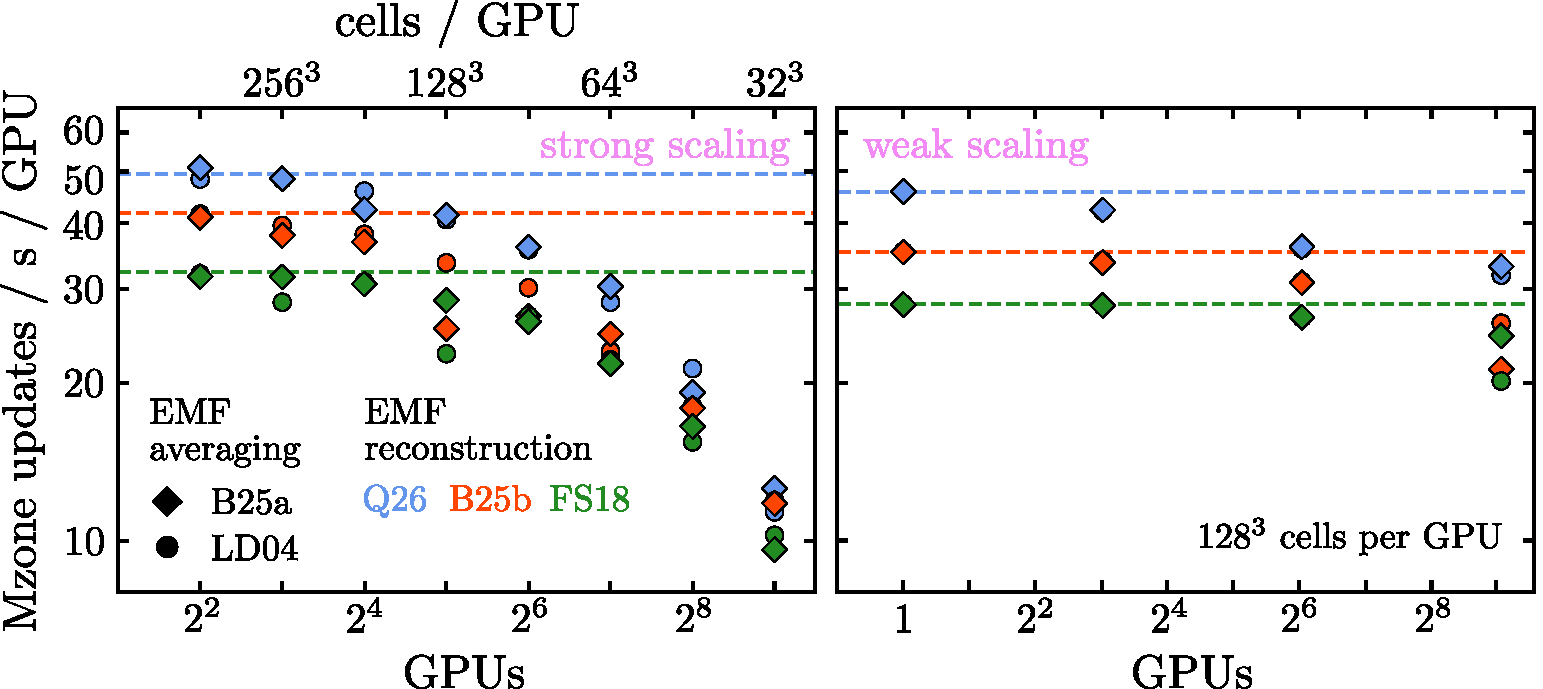
\includegraphics[width=\linewidth]{figures/quokka-mhd/results/scalings.pdf}
    \caption{Measured number of zone updates per second per GPU for all schemes as a function of GPU count, for strong scaling at fixed problem size of $512^3$ cells (left) and weak scaling at $128^3$ cells per GPU (right). Blue, green, and red points show the Q26, \citetalias{Balsara25a}, and \citetalias{Felker18a} EMF reconstruction schemes, while circles and squares show \citetalias{Londrillo04a} and \citetalias{Balsara25b} EMF averaging, respectively. Dashed horizontal lines indicate perfect scaling for each scheme.}
    \label{fig:scalings}
\end{figure}

To evaluate the speed of the MHD schemes, we carry out tests of both weak and strong scaling. The test problem we use is a non-grid aligned linear Alfv\'en wave with $\tilde{\mVector{k}} = \{1,2,3\}$ and $\theta = \pi / 4$, and we solve this problem using the same combinations of reconstruction scheme, averaging scheme, and interpolation method as in \autoref{sec:performance:waves}. In all cases we evolve the initial configuration for 100 time steps and measure the speed excluding startup and I/O. For the weak scaling test we use a domain of size $(128 \times N_\mathrm{GPU}^{1/3})^3$ for GPU counts of $N_\mathrm{GPU} \in \{1, 8, 64, 512\}$, so that the number of cells per GPU is fixed at $128^3$. For strong scaling we use a fixed problem size of $512^3$ cells, and test performance at GPU counts of $N_\mathrm{GPU} = 4$ to $512$ in factor of two steps; we do not carry out strong scaling tests on fewer than four GPUs due to memory size limitations. Thus our strong scaling test uses counts of cells per GPU ranging from $\approx 323^3$ at 4 GPUs to $64^3$ at 512 GPUs.

We report the results of our weak scaling tests in \autoref{tab:weak_scaling_zone_update_times_ngpu} and our strong scaling tests in \autoref{tab:strong_scaling_zone_update_times_ngpu}, and plot both results together in \autoref{fig:scalings}. Our figure of merit for these tests is the cell advance time $t_\mathrm{adv}$, defined as the amount of GPU compute time required to advance one cell for one time step, and its inverse the advance rate per GPU, $\Gamma = 1/t_\mathrm{adv}$ -- smaller $t_\mathrm{adv}$ and larger $\Gamma_\mathrm{adv}$ are better. These results enable us to make a few observations.

First, the Q26 EMF reconstruction scheme is consistently the fastest across all tests, followed by \citetalias{Balsara25a} and then \citetalias{Felker18a}. The speed advantage is significant: Q26 is $\approx 1.3\times$ faster than the \citetalias{Balsara25a} scheme and $\approx 1.6\times$ faster than the \citetalias{Felker18a} scheme. These differences persist across node count for both weak and strong scaling, with the exception of strong scaling at the largest node count, where the number of cells per GPU is well below our optimal count (see below).

Second, the EMF averaging scheme has almost no effect on the speed. the reconstruction scheme and reconstruction order are important, but the way that the EMFs are combined at cell corners is not. Again, this is true at all GPU counts and for both weak and strong scaling.

Third, regardless of scheme, the code shows good scaling. Almost all schemes achieve better than 70\% weak scaling efficiency\footnote{
    Here we use the usual definition of scaling efficiency, $\epsilon(N_\mathrm{GPU}) = t_\mathrm{adv,min} / t_\mathrm{adv}(N_\mathrm{GPU})$, where $t_\mathrm{adv,min}$ is the advance time on the minimum number of GPUs tested.
} going from 1 to 512 GPUs. The strong scaling efficiency is similarly better than 70\% as long as the number of cells per GPU is $128^3$ or more (corresponding to $N_\mathrm{GPU}=64$ for our test setup). We only see significant scaling efficiency loss at smaller cell counts.

\subsection{Summary and recommendations}
\label{sec:performance:summary}

For EMF reconstruction, our tests show that our newly-introduced Q26 scheme offers the highest speeds and produces results in both linear and non-linear problems that are as good as the existing \citetalias{Felker18a} and \citetalias{Balsara25a} schemes. Its only downside is that it appears to be slightly less stable when combined with higher-order reconstruction methods such as PPM or PPM-EP, and thus may prove unusable for very challenging problems at high order. By contrast the choice of EMF averaging scheme -- \citetalias{Londrillo04a} versus \citetalias{Balsara25b} -- appears to make little difference to speed, accuracy, or stability. All our comparisons of averaging scheme produce nearly identical results. 

Based on these findings, our recommendation, which we adopt as the default in \textsc{Quokka}, is to use Q26 EMF reconstruction together with \citetalias{Balsara25a} EMF averaging as the first line method. This is the fastest option by a substantial margin. If this proves to be unstable, one can fall back on \citetalias{Balsara25b} EMF reconstruction instead, which is the second-fastest, and is more stable.

\section{Tests for the recommended scheme}
\label{sec:tests}

In this Section we subject or recommended scheme to a series of additional tests that stress various parts of the algorithm. We use our recommended combination of Q26 reconstruction plus \citetalias{Balsara25a} averaging with PPM-EP interpolation for all the tests presented here unless otherwise noted.

\subsection{Non-grid aligned linear waves}
\label{sec:tests:misaligned-waves}

We start by demonstrating that our recommended scheme accurately evolves linear waves when they are not aligned with the grid. To this end, we simulate Alfv\'en, fast, and slow MHD waves. The first two of these use the same framework introduced in \autoref{sec:performance:waves}, where the slow wave was not previously tested, and has an analogous setup, where the perturbed state is of the form
\begin{align}
    &\delta\mVector{S}_\mathrm{c}^{\{\mathrm{sm}\}}
        = \delta_{a} \cos\sbrac{\omega t - \mVector{k}\cdot\mVector{x}}
        \nonumber \\
        &\nquad[1] \begin{Bmatrix}
            \phi_1 \rho_0 \\
            c_\mathrm{sm} (
                    -\phi_1 \mVectorUnit{n}_{k}
                    + \phi_2 \mVectorUnit{n}_\perp
                ) \\
            \phi_1 p_0 \gamma / (\gamma-1)
                + b_0^2\sin\theta
                + \delta_{a} \rbrac{
                        b_0^2 / 2
                        + \rho_0 c_\mathrm{sm}^2 (\phi_1^2 + \phi_2^2)
                    } \\
            b_0 \mVectorUnit{n}_\perp
        \end{Bmatrix}
    ,
\end{align}
where $\mVectorUnit{n}_\perp$ is a unit vector orthogonal to $\mVectorUnit{n}_{k}$ and lying in the plane formed by $\mVectorUnit{n}_{k}$ and $\mVectorUnit{n}_{0}$, 
\begin{align}
    c_\mathrm{sm}^2
        = \frac{1}{2}\rbrac{
            c_\mathrm{s}^2
            + c_\mathrm{A}^2
            - \rbrac{
                    \rbrac{c_\mathrm{s}^2
                    + c_\mathrm{A}^2}^2
                    - 4 c_\mathrm{s}^2 c_\mathrm{A}^2 \cos^2\theta
                }^{1/2}
        }
\end{align}
is the slow magnetosonic wave speed and the geometric factors $\phi_1$ and $\phi_2$ are
\begin{align}
    \phi_1
        &= \frac{
            c_\mathrm{sm}^2 - c_\mathrm{A}^2\cos^2\theta
        }{
            c_\mathrm{sm}^2 \sin\theta
        } \\
    \phi_2
        &= \rbrac{\frac{c_\mathrm{A}}{c_\mathrm{sm}}}^2 \cos\theta
    .
\end{align}

For our tests of non-grid aligned waves, we choose $\tilde{\mVector{k}} = \{1,2,3\}$ and $\theta = \pi / 4$ for all wave types, and simulate for a time $t = 4\pi/\omega$ (\ie two wave periods) in a domain of $512^3$ cells. Thus neither the wave vector nor the background magnetic field are aligned with any of the cardinal axes. All other parameters are identical to those used in \autoref{sec:performance:waves}, and we also measure the $L_1$ error for our solutions exactly as in that Section.

As a representative example, we plot the pencil profiles of the $b_1$ component of the magnetic field for the slow wave, in \autoref{fig:slow-waves}. The slow wave is the most stringent of the three linear wave modes, since its velocity and magnetic perturbations are oblique, compressive, and coupled, so any directional bias in the numerical fluxes would manifest as phase drift or errors in the wave-amplitude. As we show in the pencil profiles, however, after two wave periods, the solution maintains excellent conservation of the amplitude and phase, with an $L_1 = 4.6 \times 10^{-11}$ (at the level of floating-point precision) between the final and initial profiles, which is consistent with the errors we measured for the grid-aligned linear wave tests in \autoref{sec:performance:waves}.

\begin{figure}
    \centering
    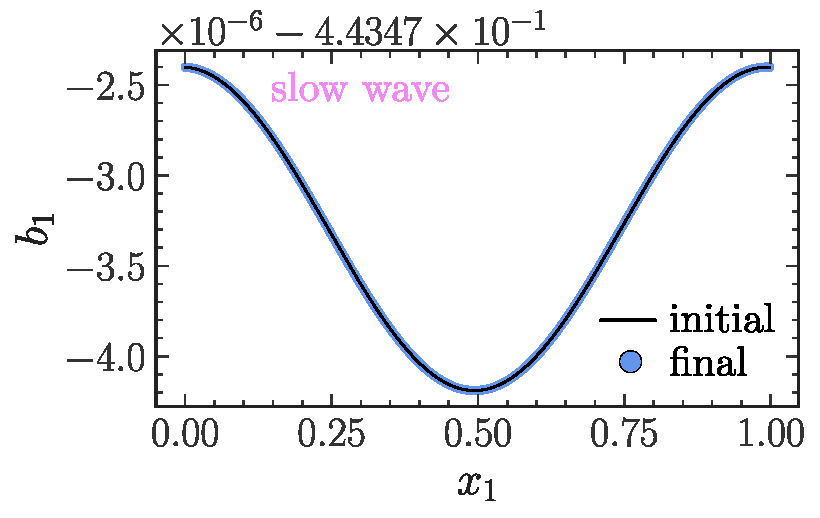
\includegraphics[width=0.65\linewidth]{figures/quokka-mhd/results/slow-Bx-along-x.pdf}
    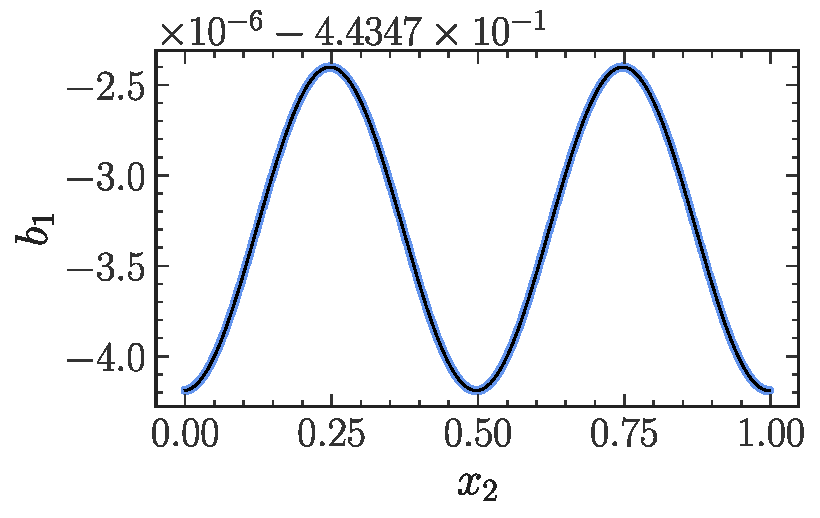
\includegraphics[width=0.65\linewidth]{figures/quokka-mhd/results/slow-Bx-along-y.pdf}
    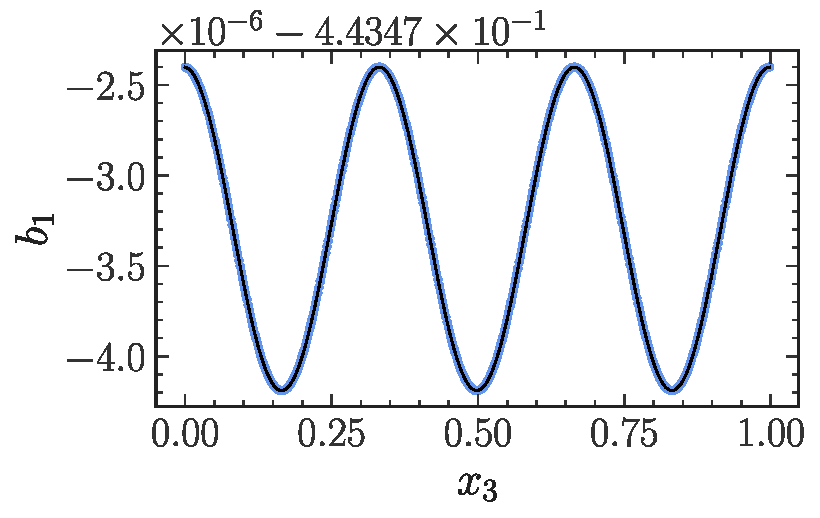
\includegraphics[width=0.65\linewidth]{figures/quokka-mhd/results/slow-Bx-along-z.pdf}
    \caption{Representative pencil profiles of the slow wave solution run with $512^3$ cells, comparing the initial profile (black line) against the solution after two wave periods (blue points). We show how the $b_1$ component of the magnetic field varies along the $x_1$ (top), $x_2$ (middle), and $x_3$ (bottom) cardinal axis.}
    \label{fig:slow-waves}
\end{figure}

% \subsection{Current sheet}

\subsection{Balsara vortex}
\label{sec:tests:balsara-vortex}

Our next test is the \citet{Balsara04a} vortex. We initialise a steady-state flow field centred in a periodic domain $\mVector{x} \in [(-5, -5, -\Delta x/2), (5, 5, \Delta x/2)]$, and advect it diagonally by adding a uniform drift velocity,
\begin{align}
    \mVector{u}(\mVector{x})
        &= \mVector{u}_\mathrm{drift} + \mVector{u}_\mathrm{vortex} \\
    \mVector{u}_\mathrm{drift}(\mVector{x})
        &= \frac{\tilde{u}}{\sqrt{2}} \rbrac{\mVectorUnit{x}_1 + \mVectorUnit{x}_2} \\
    \mVector{u}_\mathrm{vortex}(\mVector{x})
        &= \tilde{u} \rbrac{x_1 \mVectorUnit{x}_2 - x_2 \mVectorUnit{x}_1} \exp\sbrac{\frac{1 - r^2}{2}} \\
    \mVector{b}(\mVector{x})
        &= \tilde{b} \rbrac{x_1 \mVectorUnit{x}_2 - x_2 \mVectorUnit{x}_1} \exp\sbrac{\frac{1 - r^2}{2}} \\
    p(\mVector{x})
        &= p_0 + \rbrac{
                \frac{\tilde{b}^2}{2} (1 - r^2) - \frac{\rho_0 \tilde{u}^2}{2}
            } \exp\sbrac{1 - r^2} \\
    \rho(\mVector{x})
        &= \rho_0
    ,
\end{align}
where $r^2 = x_1^2 + x_2^2$. In our implementation, we adopt a background state $\rho_0 = 1$, $p_0 = 1$, and $\gamma = 5/3$, so $c_\mathrm{s} = \sqrt{\gamma p_0 / \rho_0} = \sqrt{5/3}$. We parametrise the vortex velocity amplitude as $\tilde{u} = \mathcal{M} c_\mathrm{s}$, and choose $\mathcal{M} = 0.01$. We set $\tilde{b} = \tilde{u}$ to ensure MHD force balance (\ie magnetic tension exactly balances the centrifugal force associated with the vortex).

Under these conditions, \ie $p_0 - \rho_0 \tilde{u}^2 / 2 > 0$, or equivalently $\mathcal{M} < \sqrt{2 / \gamma} = \sqrt{6/5}$, the vortex is an exact equilibrium solution of the ideal MHD equations. Thus the total kinetic, magnetic, and internal energy of the flow should remain constant over time. Checking the extent to which each of these energies is conserved is therefore a very strong diagnostic of the level of numerically induced dissipation as the vortex advects relative to the grid. It is particularly effective for testing dissipation at low $\mathcal{M}$, and thus for checking the effectiveness of the low-Mach pressure rescaling fix \citep{Minoshima21a} described in \autoref{sec:methods:flux}.

We run the test at two resolutions, $64 \times 64 \times 8$ and $128 \times 128 \times 8$, and run to time $t = 30\sqrt{2}/\tilde{u}$, long enough for the vortex to advect diagonally across the periodic domain three times. We find that our recommended scheme -- Q26 reconstruction,  \citetalias{Balsara25a} averaging, and PPM-EP interpolation -- performs exceptionally well. At $64 \times 64 \times 8$ resolution, we find that the magnetic energy at the end of the simulation is $92.5\%$ of its initial value; at $128 \times 128 \times 8$ resolution this increases to $99.5\%$. \autoref{fig:balsara-vortex} shows that the vortex maintains its shape extremely well, as well, even for the lower of our two tested resolutions. The level of energy conservation we achieve is comparable to that achieved by \citet{watt2025mitigating} using a customised MHD solver optimised for conservation in the low-$\mathcal{M}$ regime.

\begin{figure}
    \centering
    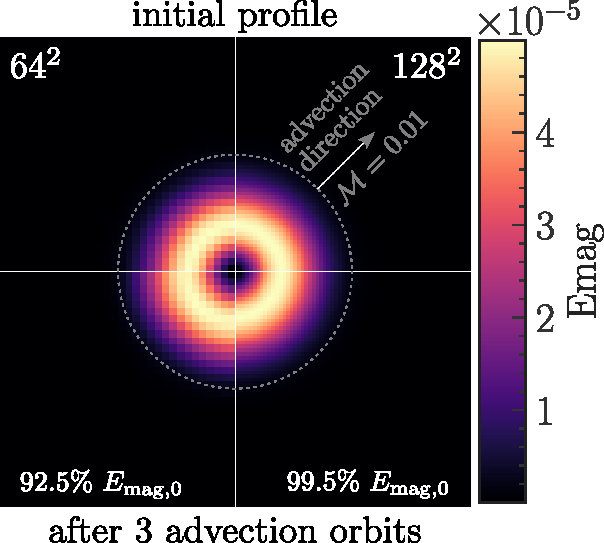
\includegraphics[width=0.65\linewidth]{figures/quokka-mhd/results/balsara-vortex.pdf}
    \caption{Slices of magnetic energy density in the Balsara vortex problem run with $\mathcal{M} = 0.01$ using Q26 reconstruction coupled with \citetalias{Balsara25a} averaging and PPM-EP reconstruction. We show the simulation run at $64 \times 64 \times 8$ on the left and at $128 \times 128 \times 8$ on the right; we show the initial condition in the top two panels, and the state after $3$ advection periods in the bottom panels. The direction of advection is shown with an arrow, and a reference circle to highlight how well the vortex maintains its shape. We also indicate the fraction of magnetic energy that is conserved.}
    \label{fig:balsara-vortex}
\end{figure}

% \subsection{Small-scale dynamo}
    
\section{Chapter Conclusions}
\label{sec:conclusions}

In this paper we have implemented ideal MHD into \textsc{Quokka}, extending its GPU-native radiation-hydrodynamic framework to magnetised flows. Our implementation couples to the existing Godunov finite-volume update of cell-centred state variables via a constrained transport (CT) update that stores magnetic fields on cell faces, using a staggered mesh 
(see \autoref{fig:schematic:grid}) that ensures $\nabla\cdot\mVector{b} = 0$ (to numerical precision) by construction. For the fluxes on these faces, we use a HLLD Riemann solver with stability and low-$\mathcal{M}$ pressure fixes based on \citet{Minoshima21a} (see \autoref{sec:methods:flux}), and develop a first-order flux correction (FOFC) strategy that improves stability by detecting cells whose high-order update would produce an unphysical state and locally falling back to a more dissipative first-order update (see \autoref{sec:methods:time-stepping}).

We break our CT scheme (see \autoref{sec:methods:emf}) up into two modular parts: (i) how the edge-centred EMFs are reconstructed from neighbouring face- and cell-centred data (see \autoref{sec:methods:emf:reconstruction}), and (ii) how the four estimates for the EMF around each edge are combined into a single upwinded value (see \autoref{sec:methods:emf:averaging}). For the EMF reconstruction step we implemented the algorithms proposed by both \citetalias{Felker18a} and \citetalias{Balsara25a} (see Schematics~\ref{fig:schematic:fs18} and \ref{fig:schematic:b25}, respectively), alongside a new strategy introduced in this paper (Q26; see Schematic~\ref{fig:schematic:q26}) that reconstructs EMFs from the velocities on cell faces deduced directly from the Riemann problem solution on those faces; this reduces the number of interpolation operations and temporary variables required to reconstruct EMFs on cell-edges. We also implemented two EMF averaging strategies, namely those of \citetalias{Londrillo04a} and \citetalias{Balsara25b}.

To determine which combination of these EMF reconstruction and EMF averaging schemes best align with \textsc{Quokka}'s performance goals (see \autoref{sec:intro:goals} for a discussion), we perform a rigorous and systematic comparison (\autoref{sec:performance}) of the accuracy and efficiency of every combination of EMF reconstruction and averaging together with three interpolation methods: piecewise linear (PLM), piecewise parabolic (PPM), and extrema-preserving PPM (PPM-EP). We test the schemes against both linear and highly-nonlinear problems, and compare not only accuracy and stability but also speed and scaling. Based on this systematic comparison, we recommend our Q26 EMF reconstruction scheme coupled with \citetalias{Balsara25a} and PPM-EP as the default configuration for \textsc{Quokka}. This combination provides the best overall balance of accuracy, stability, and GPU-efficiency across flow conditions from simple and smooth to turbulent and instability driven, and is noticeably faster than any alternatives. If better robustness is required, we recommend exchanging Q26 with \citetalias{Balsara25b}, which provides improved stability at the price of being $\approx 1.3\times$ slower. We show that our recommended scheme passes a number of other standard tests, with excellent performance (see \autoref{sec:tests}).

The ideal MHD framework implemented in this paper provides a robust and efficient module ready for scientific use, and provides a platform for future extensions. A natural next step is to incorporate explicit physical dissipation into \textsc{Quokka}, including both shear and bulk viscosity in the momentum equation (as was done in \citealt{beattie2025taking}) and Ohmic dissipation in the induction equation. These extensions would allow for controlled simulations of MHD turbulence, where dissipation effects directly affect the transport of energy and coupling of magnetic and velocity fields. In addition to this, we plan to implement a slow-shock stability fix in the HLLD Riemann solver to improve the stability of the Q26 reconstruction scheme when coupled to higher-order interpolation.

\section{Chapter End Matter}

\subsection{A Note on Notation}
\label{sec:notation}

\paragraph*{Field and index conventions.}
We use lower-case symbols for scalar and vector fields, and upper-case symbols for collections (\eg the state vector; see \autoref{defn:state-vector}) and for rank-2 tensors. Spatial indices $i$, $j$, and $k$ denote mesh positions: integers refer to cell centres, and half-integers to faces or edges (see \autoref{fig:schematic:grid}). Numbered subscripts indicate vector components aligned with coordinate axes; in three dimensions these correspond to the $x_1$, $x_2$, and $x_3$ directions, which follow the usual right-hand rule. Sub- and superscripts are also used to indicate context-specific information.

\paragraph*{Brackets and superscripts.}
Round brackets denote grouping, \eg~$a(b+c)$. Square brackets indicate evaluation at a discrete time level, $\mVector{S}^{[n]}$, $\mVector{S}^{[n+1/2]}$, and $\mVector{S}^{[n+1]}$. Curly brackets denote collections, such as the components of a vector. Superscripts are used in three ways: (i) to indicate time levels, as above; (ii) to distinguish reconstructed variants, in which case contextual information is enclosed in curly brackets, $\varepsilon_{3}^{\cbrac{TL}}\EvalAtH{i + 1/2}{j + 1/2}{k}$ and $\varepsilon_{3}^{\cbrac{BR}}\EvalAtH{i + 1/2}{j + 1/2}{k}$ and (iii) in the usual sense to denote powers (though this usage is rare in this paper).

\paragraph*{Directional splitting and interface notation.}
Because our update is directionally split, we describe the algorithm through the flux across the $x_1$-oriented face; the corresponding expressions for the $x_2$- and $x_3$-faces follow by cyclic permutation of the $i$, $j$, and $k$ indices. For clarity, we therefore work locally in the two-dimensional plane spanned by $x_1$ and $x_2$.

In reconstruction, interface states are labelled as left ($L$) and right ($R$), or top ($T$) and bottom ($B$). We denote side-based states by $S_\mathrm{I} \in \{L, R\}$ and $S_\mathrm{II} \in \{T, B\}$, and quadrant-based states either as single-sided labels $Q_\mathrm{I} \in \{T, R, B, L\}$ (for example, face-centred quantities reconstructed to a cell edge; see \autoref{fig:schematic:q26}), or as corner combinations $Q_\mathrm{II} \in \{TL, TR, BR, BL\}$ (for example, cell-centred quantities reconstructed to a cell edge; see \autoref{fig:schematic:fs18}). When necessary, we explicitly indicate reconstruction order or direction, for example $u_1^{\{Q_\mathrm{II}: x_1 x_2\}}$ and $u_1^{\{Q_\mathrm{II}: x_2 x_1\}}$.
